\chapter{Progettazione e codifica}
\label{cap:progettazione-codifica}

\intro{In questo capitolo saranno  descritte le attività di progettazione e codifica dell'applicativo.
Inoltre verranno descritte le tecnologie utilizzate durante lo sviluppo del progetto, le scelte architetturali e i componenti sviluppati.
}

\section{Tecnologie utilizzate}
\label{sec:tecnologie-strumenti}

Di seguito viene data una panoramica delle tecnologie utilizzate durante lo sviluppo del progetto di stage.

\subsection{Frontend}\label{subsec:frontend}
\subsubsection{Vue.js}\label{subsubsec:vue}
Vue.js è un framework JavaScript progressivo e reattivo, utilizzato per lo sviluppo di interfacce utente dinamiche e moderne. 
Creato da Evan You, Vue.js è apprezzato per la sua semplicità d'uso e flessibilità. Con un sistema di reattività basato su un modello di oggetti e dipendenze, 
Vue.js rende facile il monitoraggio e l'aggiornamento automatico dell'interfaccia utente in base ai cambiamenti di stato dei dati. La sua architettura basata 
su componenti consente di organizzare il codice in moduli riutilizzabili e autonomi, semplificando la creazione di applicazioni complesse. 
Grazie alle direttive, è possibile arricchire il DOM con funzionalità reattive, mentre il sistema di routing agevola la creazione di single page applications. 
Con una crescita costante della comunità di sviluppatori, Vue.js è diventato un'opzione popolare nel mondo dello sviluppo frontend.
Per il mio progetto sono andato ad utilizzare la versione 3 di Vue.js, insieme allo script setup, che è una nuova sintassi per definire componenti progettata per semplificare la struttura del codice e migliorare la leggibilità.

\subsubsection{TypeScript}\label{subsubsec:TypeScript}
TypeScript è un linguaggio di programmazione open-source sviluppato da Microsoft. Si basa su JavaScript e offre tipizzazione statica opzionale, 
consentendo agli sviluppatori di specificare tipi per variabili, parametri di funzioni e oggetti. Questa caratteristica aiuta a individuare errori e a migliorare 
la manutenibilità del codice.\\
All'interno del mio progetto sono andato a creare per la parte frontend una cartella chiamata types che contiene un file TypeScript contenente tutti i tipi utilizzati all'interno del progetto.
\subsubsection{Vite.js}\label{subsubsec:vite}
Vite.js è un build tool utilizzato per lo sviluppo di applicazioni web. È stato creato da Evan You, lo stesso creatore di Vue.js, e si basa su rollup.js.
Vite.js è stato progettato per essere veloce, semplice da utilizzare e facile da configurare. La sua velocità è dovuta al fatto che utilizza la tecnica dell'ESM (ECMAScript Modules) 
che permette di caricare i moduli in modo asincrono, riducendo i tempi di compilazione e di hot-reload.
\subsubsection{Sass}\label{subsubsec:Sass}
Sass è un'estensione di CSS che offre funzionalità aggiuntive e avanzate per semplificare e organizzare il modo in cui viene scritto e gestito il codice CSS.
Può essere considerato un preprocessore CSS, in quanto viene compilato in CSS prima di essere interpretato dal browser. Sass inoltre permette di utilizzare funzionalità non disponibili in CSS nativo, offrendo una serie di funzioni, variabili, mixin e altro.\\
Insieme a Sass, ho utilizzato BEM, ovvero una metodologia di naming convention utilizzata nel mondo dello sviluppo web.

\subsection{Backend}\label{subsec:backend}
\subsubsection{Nest.js}\label{subsubsec:nest}
Nest.js è un framework per applicazioni server-side basato su Node.js. Si basa su Express.js e TypeScript ed è progettato per creare applicazioni scalabili e performanti.
Il framework NestJS combina concetti e caratteristiche provenienti da diversi paradigmi di sviluppo, tra cui la programmazione orientata agli oggetti (OOP), la programmazione funzionale e la programmazione reattiva.

\subsection{Altre tecnologie di supporto}\label{subsec:altre-tecnologie-di-supporto}
\subsubsection{Node.js}\label{subsubsec:node.js}
Node.js è un ambiente di runtime JavaScript open-source progettato per eseguire codice lato server. Per gestire le dipendenze del mio progetto,
ho deciso di utilizzare pnpm come gestore di pacchetti. Questa selezione ha portato a un miglior utilizzo delle risorse di sistema e ha notevolmente accelerato il processo di 
installazione delle dipendenze.
 \subsubsection{Pinia}\label{subsubsec:pinia}
Pinia è una libreria per la gestione dello stato per applicazioni Vue.js. Promuove l'uso di store modulari, ognuno dei quali gestisce uno stato specifico dell'applicazione.
\subsubsection{Vue router}\label{subsubsec:vue-router}
Vue-router è una libreria per la gestione delle route per le applicazione Vue.js. Permette di definire le route dell'applicazione e di navigare tra le pagine.

\subsection{Versionamento}\label{subsec:versionamento}
\subsubsection{Git}\label{subsubsec:git}
Git è un sistema di controllo versione distribuito e altamente flessibile, utile per tenere traccia delle modifiche apportate al codice sorgente durante lo sviluppo di un progetto software.
\subsubsection{CodeCommit}\label{subsubsec:CodeCommit}
AWS CodeCommit rappresenta un servizio di hosting di repository altamente scalabile, che è gestito all'interno dell'ecosistema di Amazon Web Services (AWS). 
Con CodeCommit, è possibile ospitare repository Git privati in un ambiente sicuro e flessibile.

\subsection{Verifica}\label{subsec:verifica}
\subsubsection{ESLint}\label{subsubsec:eslint}
ESLint è uno strumento open-source ampiamente utilizzato per l'analisi statica del codice JavaScript. Esso permette di identificare e segnalare potenziali errori o pratiche non conformi durante la fase di sviluppo.
\subsubsection{Vitest}\label{subsubsec:vitest}
Vitest è un framework per l'implementazione di test di unità, utilizzato maggiormente in progetti Vue.js.
Usato in coppia con Vite permette di eseguire test di unità in modo più veloce e semplice.

\subsection{Librerie esterne utilizzate}\label{subsec:librerie-esterne}
\subsubsection{THRON Components}\label{subsubsec:thron-components}
Libreria THRON contenente i componenti del design system aziendale. Questa libreria è stata utilizzata per la creazione di componenti comuni come bottoni, del portale.
\subsubsection{Azure MSAL}\label{subsubsec:azure-MSAL}
Azure MSAL è una libreria che permette di integrare il login con Azure Active Directory all'interno di un'applicazione web.
\subsubsection{Swagger UI}\label{subsubsec:swagger-ui}
Swagger UI è una libreria open-source progettata per semplificare la visualizzazione e l'interazione con la documentazione delle API.

\section{Struttura principale del sistema}
Il sistema è composto da due principali sezioni:
\begin{itemize}
  \item Frontend, ovvero l'interfaccia utente dell'applicazione web che permette all'utilizzatore di interagire con il sistema. È responsabile di presentare i contenuti in modo visivamente attraente e interattivo, consentendo agli utenti di navigare, inserire dati e svolgere azioni specifiche. Per lo
  sviluppo di questa parte del sistema è stato utilizzato il framework Vue.js;
  \item Backend, ovvero la parte del sistema che elabora le richieste provenienti dal frontend e restituisce i risultati. È responsabile della gestione dei dati e della logica di business.
  Lo sviluppo di questa parte del sistema è stato realizzato utilizzando il framework Nest.js. 
\end{itemize}

\subsection{Ambienti di sviluppo}
Gli ambienti di staging sono ambienti di test che vengono utilizzati per testare le funzionalità dell'applicazione prima di rilasciarla in produzione.
% A livello aziendale sono stati definiti tutte e tre come ambienti di staging e sono stati denominati come segue:
A livello aziendale sono stati definiti tre ambienti di cui i primi due di staging, denominati come segue:
\begin{itemize}
  \item \textbf{Development}: consente di validare a livello tecnico le funzionalità;
  \item \textbf{Quality}: consente di validare a livello funzionale o di implementazione delle funzionalità;
  \item \textbf{Production}: ambiente di produzione in cui viene rilasciata la funzionalità.
\end{itemize}

\subsection{Configurazione ambiente del progetto}
Il progetto di stage, necessita di cartelle per la configurazione dell'ambiente di sviluppo, per la configurazione del progetto e per la configurazione del deploy.
Più precisamente, il progetto segue la seguente struttura:

\subsubsection*{\emph{Buildspec}}
La cartella buildspec contiene i file di configurazione per la build dell'applicazione su AWS CodeBuild.
Questo è il primo step del processo di deploy, in quanto viene eseguito la build sia del middleware che del portale.
La cartella è formata a sua volta da tre file: buildspec\_development, buildspec\_quality e buildspec\_production. 
Ognuno di questi file configura la build dell'applicazione in base all'ambiente di deploy.\\
Successivamente dopo aver effettuato tutti i comandi specificati nei file buildspec, inizia lo step di deploy, specificato nella cartella Infra.
Ognuno dei file buildspec è un file YAML, che è formato dalle seguenti sezioni:
\begin{itemize}
  \item La sezione env dove vengono specificate le variabili d'ambiente utilizzate nel progetto;
  \item La sezione di pre-build dove vengono specificati i comandi da eseguire prima della build;
  \item La sezione di build dove vengono specificati i comandi per la build del portale e del middleware.
\end{itemize}

\subsubsection*{\emph{Infra}}
La cartella Infra contiene i file di configurazione per il deploy dell'applicazione su AWS. È scritta utilizzando il linguaggio di programmazione Python.\\
La cartella è formata da due file: app.py e stack.py. Il primo file contiene la configurazione per il deploy dell'applicazione, mentre il secondo file contiene la configurazione per il deploy dell'infrastruttura.\\
Per quanto riguarda l'infrastruttura del progetto, sono andato ad utilizzare e a configurare due costrutti, anche chiamati CDK Constructs o semplicemente Constructs, che sono delle classi che rappresentano un componente dell'infrastruttura.
Il primo costrutto si chiama THRONCloudFrontDistribution e consente di accelerare la distribuzione dei contenuti web statici e dinamici, come file .html, .css, .js e immagini, agli utenti.
In breve questo costrutto genera il template di AWS CloudFront ed esegui il deploy degli asset statici su un bucket S3.\\
Il secondo costrutto che sono andato ad utilizzare si chiama THRONDockerLambda e consente di creare una funzione lambda in cui il gestore è un'immagine docker.
Nel caso del mio progetto, mi è servito per creare un lambda che una volta invocata avvia un docker con all'interno il progetto backend.\\

\subsection*{\emph{Middleware}}
La cartella Middleware contiene il progetto backend in Nest-js. Nello specifico la cartella è formata dalle seguenti sezioni:
\begin{itemize}
  \item La cartella src che contiene il codice sorgente dell'applicazione, dove vengono specificati i vari endpoint che utilizzo sulla parte frontend, lo script per il setting
  della lambda, una cartella con gli helpers e la cartella del middleware.
  \item La cartella test che contiene i test di unità dell'applicazione;
  \item File env che contiene le variabili d'ambiente utilizzate nel progetto;
  \item Una cartella node\_modules che contiene le dipendenze del progetto.
\end{itemize}
\subsection*{\emph{Portal}}
La cartella portal contiene il progetto frontend in vue-js. Nello specifico la cartella è formata dalle seguenti sezioni:
\begin{itemize}
  \item La cartella public che contiene il file index.html, che è il file principale dell'applicazione;
  \item Una cartella node\_modules che contiene le dipendenze del progetto;
  \item La cartella src che contiene il codice sorgente dell'applicazione, dove vengono specificati i vari componenti che utilizzo, i vari store, i vari router e i vari utils.
  \item File env che contiene le variabili d'ambiente utilizzate nel progetto.
\end{itemize}

\subsection*{\emph{Dockerfile}}
Il file Dockerfile è un file docker che contiene le istruzioni per creare un'immagine che verrà utilizzata per eseguire il middleware all'interno di una lambda.\\
Utilizzando la struttura Dockerfile, sono andato a creare un ambiente isolato in cui il middleware può essere configurato e utilizzato come parte della mia funzione 
lambda. Quando la funzione viene invocata, avvia il Docker container ed esegue il middleware all'interno dell'ambiente containerizzato, 
garantendo che esso sia parte integrante dell'applicazione serverless.

% buildspec -> cartella con configuraazione dei build, per codebuild primo step, builda sia portal che il middleware
% quando finsice la build ti attacca allo step di deploy, definite in infra. 
% PEr il portale costrutto cloudfrontdistribution -> genera il template di aws clodfront e esegue il deploy degli asset statici su s3. S3 container
% Secondo costrutto -> throndockerlambda e questo crea la lambda con quando viene invocata avvia un docker con all'interno il mio middleware.

\section{Progettazione}\label{sec:progettazione}

\subsection{Architettura frontend}\label{subsec:architettura-front-end}
\subsubsection{Architettura Vue.js}\label{subsubsec:architettura-vue.js}
Vue.js è un framework utilizzato nelle single page application, che permette di definire le pagine web in modo modulare, utilizzando componenti riutilizzabili.
I componenti costituiscono la base dell'architettura di Vue. Essi rappresentano una parte isolata dell'interfaccia, che può contenere il proprio modello, i propri stili e la propria logica, infatti ogni componente ha il proprio
template scritto in HTML, il proprio script scritto nel mio caso in TypeScript e i propri stili scritti nel mio caso in scss.
Come già accennato in precedenza, i componenti sono riutilizzabili all'interno di un'applicazione e possono essere combinati tra loro per creare gerarchie di interfaccie ancora più complesse.\\

L'architettura di Vue.js è basata sul pattern architetturale MVVM (Model-View-ViewModel), che è una variante del pattern MVC (Model-View-Controller), dove:
\begin{itemize}
  \item \textbf{Model}: rappresenta lo stato, i dati e le regole di business dell'applicazione, che gestiscono l'accesso e la modifica di tali dati. Lo stato viene definito tramite l'uso
  di particolari variabili di tipo reattivo, che permettono di aggiornare automaticamente la view associata in caso di modifiche;
  \item \textbf{View}: è l'interfaccia utente, che visualizza i dati contenuti nel model e si occupa di reagire agli input dell'utente. La view è definita utilizzando i template Vue.js e viene reattivamente aggiornata in base ai cambiamenti del modello. La vista viene definita utilizzando un template, ovvero una direttiva dell'HTML, arricchita con alcune direttive Vue.js. 
  Queste particolari direttive permettono di collegare elementi del DOM a proprietà o metodi del modello, in modo che la view possa reagire agli input dell'utente e aggiornare automaticamente lo stato dell'applicazione;
  \item \textbf{ViewModel}: è l'intermediario tra la view e  il model. Il ViewModel gestisce la logica dell'interfaccia utente e mantiene lo stato dell'applicazione sincronizzato con la view.
  Il ViewModel è rappresentato da un componente Vue.js, infatti esso è un'istanza che collega il modello e la vista. All'interno di un componente è possibile definire metodi, proprietà 
  computate, metodi del ciclo di vita, gestione di eventi e molte altre funzionalità. Questo consente di definire la logica di presentazione e di manipolare i dati all'interno di un contesto definito.
\end{itemize}

In breve, l'architettura è incentrata sulla creazione e utilizzo di componenti riutilizzabili che al loro interno incorporano sia il modello che la vista. Un aspetto che rende Vue.js
diverso da altri framework è proprio il concetto di reattività, infatti Vue.js è in grado di rilevare automaticamente le dipendenze tra i componenti, in modo da poter aggiornare automaticamente l'interfaccia utente.

\subsection{Architettura back-end}\label{subsec:architettura-backend}
\subsubsection{Architettura Nest.js}\label{subsubsec:architettura-nest.js}
L'architettura di Nest.js si basa su diversi principi chiave e concetti fondamentali che lo rendono un framework efficace per la creazione di applicazioni server-side.
La caratteristica principale di Nest.js è la modularità, che promuove la suddivisione dell'applicazione in moduli, consentendo di organizzare il codice in unità funzionali e riutilizzabili.\\
Di seguito i concetti base su cui si basa l'architettura:
\begin{itemize}
  \item \textbf{Module}: rappresenta un'unità organizzativa dell'applicazione che contiene un gruppo di elementi correlati come controller, service e provider. Questa struttura modulare 
  favorisce la separazione delle responsabilità rendendo il codice più leggibile;
  \item \textbf{Controller}: sono interfacce tra la rete e la logica dell'applicazione responsabili della gestione delle richieste HTTP in ingresso. Ogni controller è associato a un percorso specifico e a uno o più metodi che rappresentano le diverse azioni eseguibili sul percorso;
  \item \textbf{Service}: contiene la logica di business dell'applicazione. I service sono responsabili della gestione dei dati e dell'interazione con le risorse esterne.
\end{itemize}

% \paragraph{}\label{par:}

\section{Codifica}
In questa sezione vengono descritti i componenti e le funzionalità sviluppate durante il progetto di stage. 
Per questioni di chiarezza e di ordine, questa sezione è suddivisa in due parti: la prima rappresenta la parte frontend, mentre la seconda rappresenta la parte backend.
\subsection{Codifica frontend}\label{subsec:codifica-front-end}

\subsubsection{Utils}\label{subsubsec:utils}
La cartella Utils contiene una serie di file TypeScript che rappresentano funzioni, utilities o moduli che forniscono funzionalità di supporto a varie parti dell'applicazione.
Questi file sono progettati per semplificare compiti ripetitivi, astrazioni complesse o per fornire funzionalità condivise in più componenti. Ogni utils è accompagnato 
da un file di test che ne verifica il corretto funzionamento.\\
Di seguito sono elencati gli utils che ho sviluppato durante il progetto di stage.

\paragraph{Auth}\label{par:auth-utils}
Il file Auth è una utility per la gestione dell'autenticazione utilizzando come supporto la libreria Azure MSAL. Essa è utile
per interfacciarsi all'autenticazione verso il servizio Azure Active Directory.\\
Auth è composto da più metodi, a partire dalla funzione di login fino alla funzione di acquisizione del token di accesso.\\
Una funzione importante che ho implementato con l'aiuto della libreria \textit{Azure MSAL} è la funzionalità di recupero del token in modo automatico con 
l'implementazione del \textit{refresh token}. Essa segue la procedura seguente:
\begin{enumerate}
  \item Inanzitutto viene controllata la \textit{cache} nell'archivio del browser per verificare se esiste un token di accesso ancora valido per la sessione corrente. Se lo trova lo restituisce;
  \item In caso il token sia scaduto o non esista proprio, viene tentato l'utilizzo del \textit{refresh token} per ottenere un nuovo token di accesso;
  \item In caso siano passate ventiquattro ore, ovvero la validità del \textit{refresh token}, la libreria \textit{Azure MSAL} apre un \textit{hidden iframe} per richiedere
  un nuovo codice di autorizzazione usando la sessione corrente dell'utente se esiste, e quindi un nuovo token di accesso e di aggiornamento. 
\end{enumerate}
Questo procedimento per il recupero del token per mantenere la sessione attiva, può non funzionare correttamente nei seguenti casi:
\begin{itemize}
  \item L'utente ha cambiato la password;
  \item Il browser blocca i cookie di terze parti, che previene l'utilizzo del \textit{hidden iframe} per il recupero del token;
\end{itemize}
In questi casi, si verificherà un errore che verrà catturato tramite un \textit{try catch} e verrà utilizzato il metodo di login con pop-up per effettuare nuovamente l'autenticazione.
\paragraph{Debounce}\label{par:debounce}
Il file Debounce è una utility che ho creato per ritardare l'esecuzione di una funzione fino a quando non si verifica
un certo intervallo di tempo in cui non vengono eseguite chiamate.\\
Questa utility è stato utilizzato per ritardare l'esecuzione della chiamata POST per il filtraggio dei risultati della ricerca. 
In questo modo, quando l'utente digita nella barra di ricerca, la chiamata POST viene eseguita ogni 300 millisecondi, ignorando le chiamate precedenti.

\paragraph{EndpointApiCall}\label{par:endpoint-api-call}
L'utility EndpointApiCall è una funzione che ho creato per gestire le chiamate ai vari endpoint del middleware, per ottenere
i dati relativi alle API disponibili nel sistema.
Queste chiamate necessitano di token di autenticazione valido per la sessione corrente, necessario per evitare chiamate non autorizzate.

\paragraph{GetClients}\label{par:get-clients}
L'utils GetClients è una funzione progettata per effettuare una richiesta HTTP GET al progetto del middleware, al fine di
ottenere la lista dei client disponibili nel sistema. Questa funzione è stata utilizzata per popolare la lista dei client disponibili
per la ricerca, in modo da poter selezionarne uno tra quelli disponibili, in base all'ambiente di sviluppo.
La chiamata necessita di un token di autenticazione valido per la sessione corrente per evitare chiamate non autorizzate.

\paragraph{GetResults}\label{par:get-results}
L'utils getResults è una funzione progettata per effettuare una richiesta HTTP POST al middleware, che sono andato ad utilizzare per ritornare 
i risultati della ricerca. Infatti, la ricerca nel mio progetto è spostata lato backend, che è una best practice usata in azienda.
La chiamata è autenticata, e viene utilizzata insieme alla funzione di debounce, per ritardare l'esecuzione della chiamata POST. Come body della chiamata,
viene passato il testo che l'utente sta scrivendo nella barra di ricerca.

\paragraph{MsGraphApiCall}\label{par:ms-graph-api-call}
L'utils MsGraphApiCall contiene al suo interno due funzioni che ho creato per effettuare chiamate all'API di Microsoft Graph. 
La prima funzione è una chiamata GET, che viene utilizzata per ottenere i dati relativi all'utente che ha effettuato l'accesso al portale.
La seconda funzione è sempre una chiamata GET ad un altro endpoint di Microsoft, per ottenere informazioni secondarie sull'utente, come ad esempio l'immagine del profilo.
Entrambe le chiamate necessitano di un token, diverso dal token utilizzato per le chiamate al middleware. Infatti, questo token è specifico per le chiamate verso Microsoft Graph.

\paragraph{SwaggerUtils}\label{par:swagger-utils}
% da capire


\subsubsection{Config}\label{subsubsec:config}
\paragraph{ConfigAuth}\label{par:config-auth}
Il seguente file rappresenta un modulo di configurazione per l'autenticazione. Esso contiene le configurazioni per l'autenticazione verso Azure Active Directory,
come il clientId, il redirectUri o l'authority.  

\subsubsection{Stores}\label{subsubsec:store}
La cartella stores contiene i vari store utilizzati all'interno del progetto in Vue.js. Gli store sono utili per gestire lo stato dell'applicazione,
in modo da poterlo condividere tra più componenti.\\
Di seguito sono descritti gli store che ho sviluppato durante il progetto di stage.

\paragraph{Auth}\label{par:auth-store}
Il seguente store è stato creato per gestire lo stato dell'autenticazione utente e l'interazione con un servizio di autenticazione esterno.
Esso utilizza al suo interno l'utils Auth che ho descritto in precedenza, e contiene delle variabili reattive per la gestione dello stato dell'autenticazione
e per la gestione dei token.\\
Ho scritto lo store Auth utilizzando uno stile di programmazione basato su funzione closure di JavaScript. Questo approccio consente di incapsulare
lo stato dell'autenticazione consentendo un maggiore controllo sull'accesso alle variabili e alle funzioni all'interno del modulo.

\paragraph{Store}\label{par:store}
Il seguente store, a differenza del precedente, utilizza Pinia, una libreria apposita per la gestione dello stato.
Esso è utilizzato per la gestione delle API e client-id disponibili nell'applicazione. Infatti, lo store inizializza le variabili reattive per la gestione
delle API e dei client-id, effettuando una chiamata al middleware, utilizzando le utility apposite definite precedentemente.

\subsubsection{Router}\label{subsubsec:router}
La cartella router contiene le rotte definite nel progetto, ovvero le route che l'utente può visitare all'interno dell'applicazione e un helper per la gestione del router.
\paragraph{CustomNavigation}\label{par:custom-navigation}
Il seguente file rappresenta una classe con due metodi: il primo utilizzato nel flusso di autenticazione, più precisamente nelle richieste con pop-up,
mentre il secondo è utilizazto per convertire qualsiasi URI di reindirizzamento completoq in un URI di reindirizzamento relativo, in modo che il Vue Router
possa gestire correttamente il reindirizzamento in modo sicuro.

%%%%%%%%%%%%%%%%%%%%%%%%%%%%%%%%%%%%%%%%%%%%%%%%%%%%%%%%%%%%%%%%%%%%%%%%%%%%%%%%%%%%%%%%%%%%%%%%%%%%%%%%%%%%%%%%%%%%%%

\subsubsection{Views}\label{subsubsec:views}
La seguente sezione contiene le views, ovvero le pagine dell'applicazione.
Di seguito sono descritte le views che ho sviluppato durante il progetto di stage.

\paragraph{LoginView}\label{par:login-view}
La LoginView è la prima pagina con cui l'utente interagisce (in figura~\ref{fig:login-view}). Essa contiene un bottone che permette di effettuare il login tramite pop-up, tramite un account Microsoft 365.
La pagina consente di accedere al portale, ed è l'unica pagina di tutto il progetto che non richiede l'autenticazione.\\
Quando un'utente non autenticato tenterà di accedere a qualsiasi altra pagina del portale, verrà sempre reindirizzamento
automaticamente a questa view. La pagina al suo interno contiene un unico componente, ovvero LoginButton, che verrà descritto in seguito.
\begin{figure}[ht]
  \centering
  
\includegraphics[width=0.6\textwidth, alt={Pagina di login dell'applicazione}]{images/frontend/LoginView.jpg}
  \caption{LoginView}\label{fig:login-view}
\end{figure}
% \clearpage
\pagebreak

Inoltre, per permettere un uso comodo anche in schermi di piccole dimensioni, o comunque utilizzando una scheda del browser ristretta, ho sviluppato
un design responsive (in figura~\ref{fig:login-view-responsive}), che permette di visualizzare il contenuto in maniera ottimale anche su spazi ridotti.
Ciò secondo me è necessario perchè trattandosi di un portale per la consultazione di documentazione, è possibile che l'utente 
lo utilizzi in combinazione con altre schede del browser.

\begin{figure}[ht]
  \centering
  
\includegraphics[width=0.6\textwidth, alt={Pagina di login responsive dell'applicazione}]{images/frontend/LoginViewRes.jpg}
  \caption{LoginView responsive}\label{fig:login-view-responsive}
\end{figure}


\paragraph{HomeView}\label{par:home-view}
La seguente view rappresenta la prima pagina visibile dopo aver effettuato il login, infatti dopo che l'autenticazione si è conclusa con successo, 
l'utente viene reindirizzato a questa pagina (in figura~\ref{fig:home-view}).
La \textit{HomeView} è composta da tre sezioni principali: \textit{HeaderNav}, \textit{Sidebar} e \textit{StartPage}. Quest'ultimo è il componente visibile 
subito dopo aver effettuato il login. Infatti quando l'utente inizierà a navigare tra le varie \textit{API}, la \textit{StartPage} verrà sostituita con il \textit{MainContent}.

\begin{figure}[ht]
  \centering
  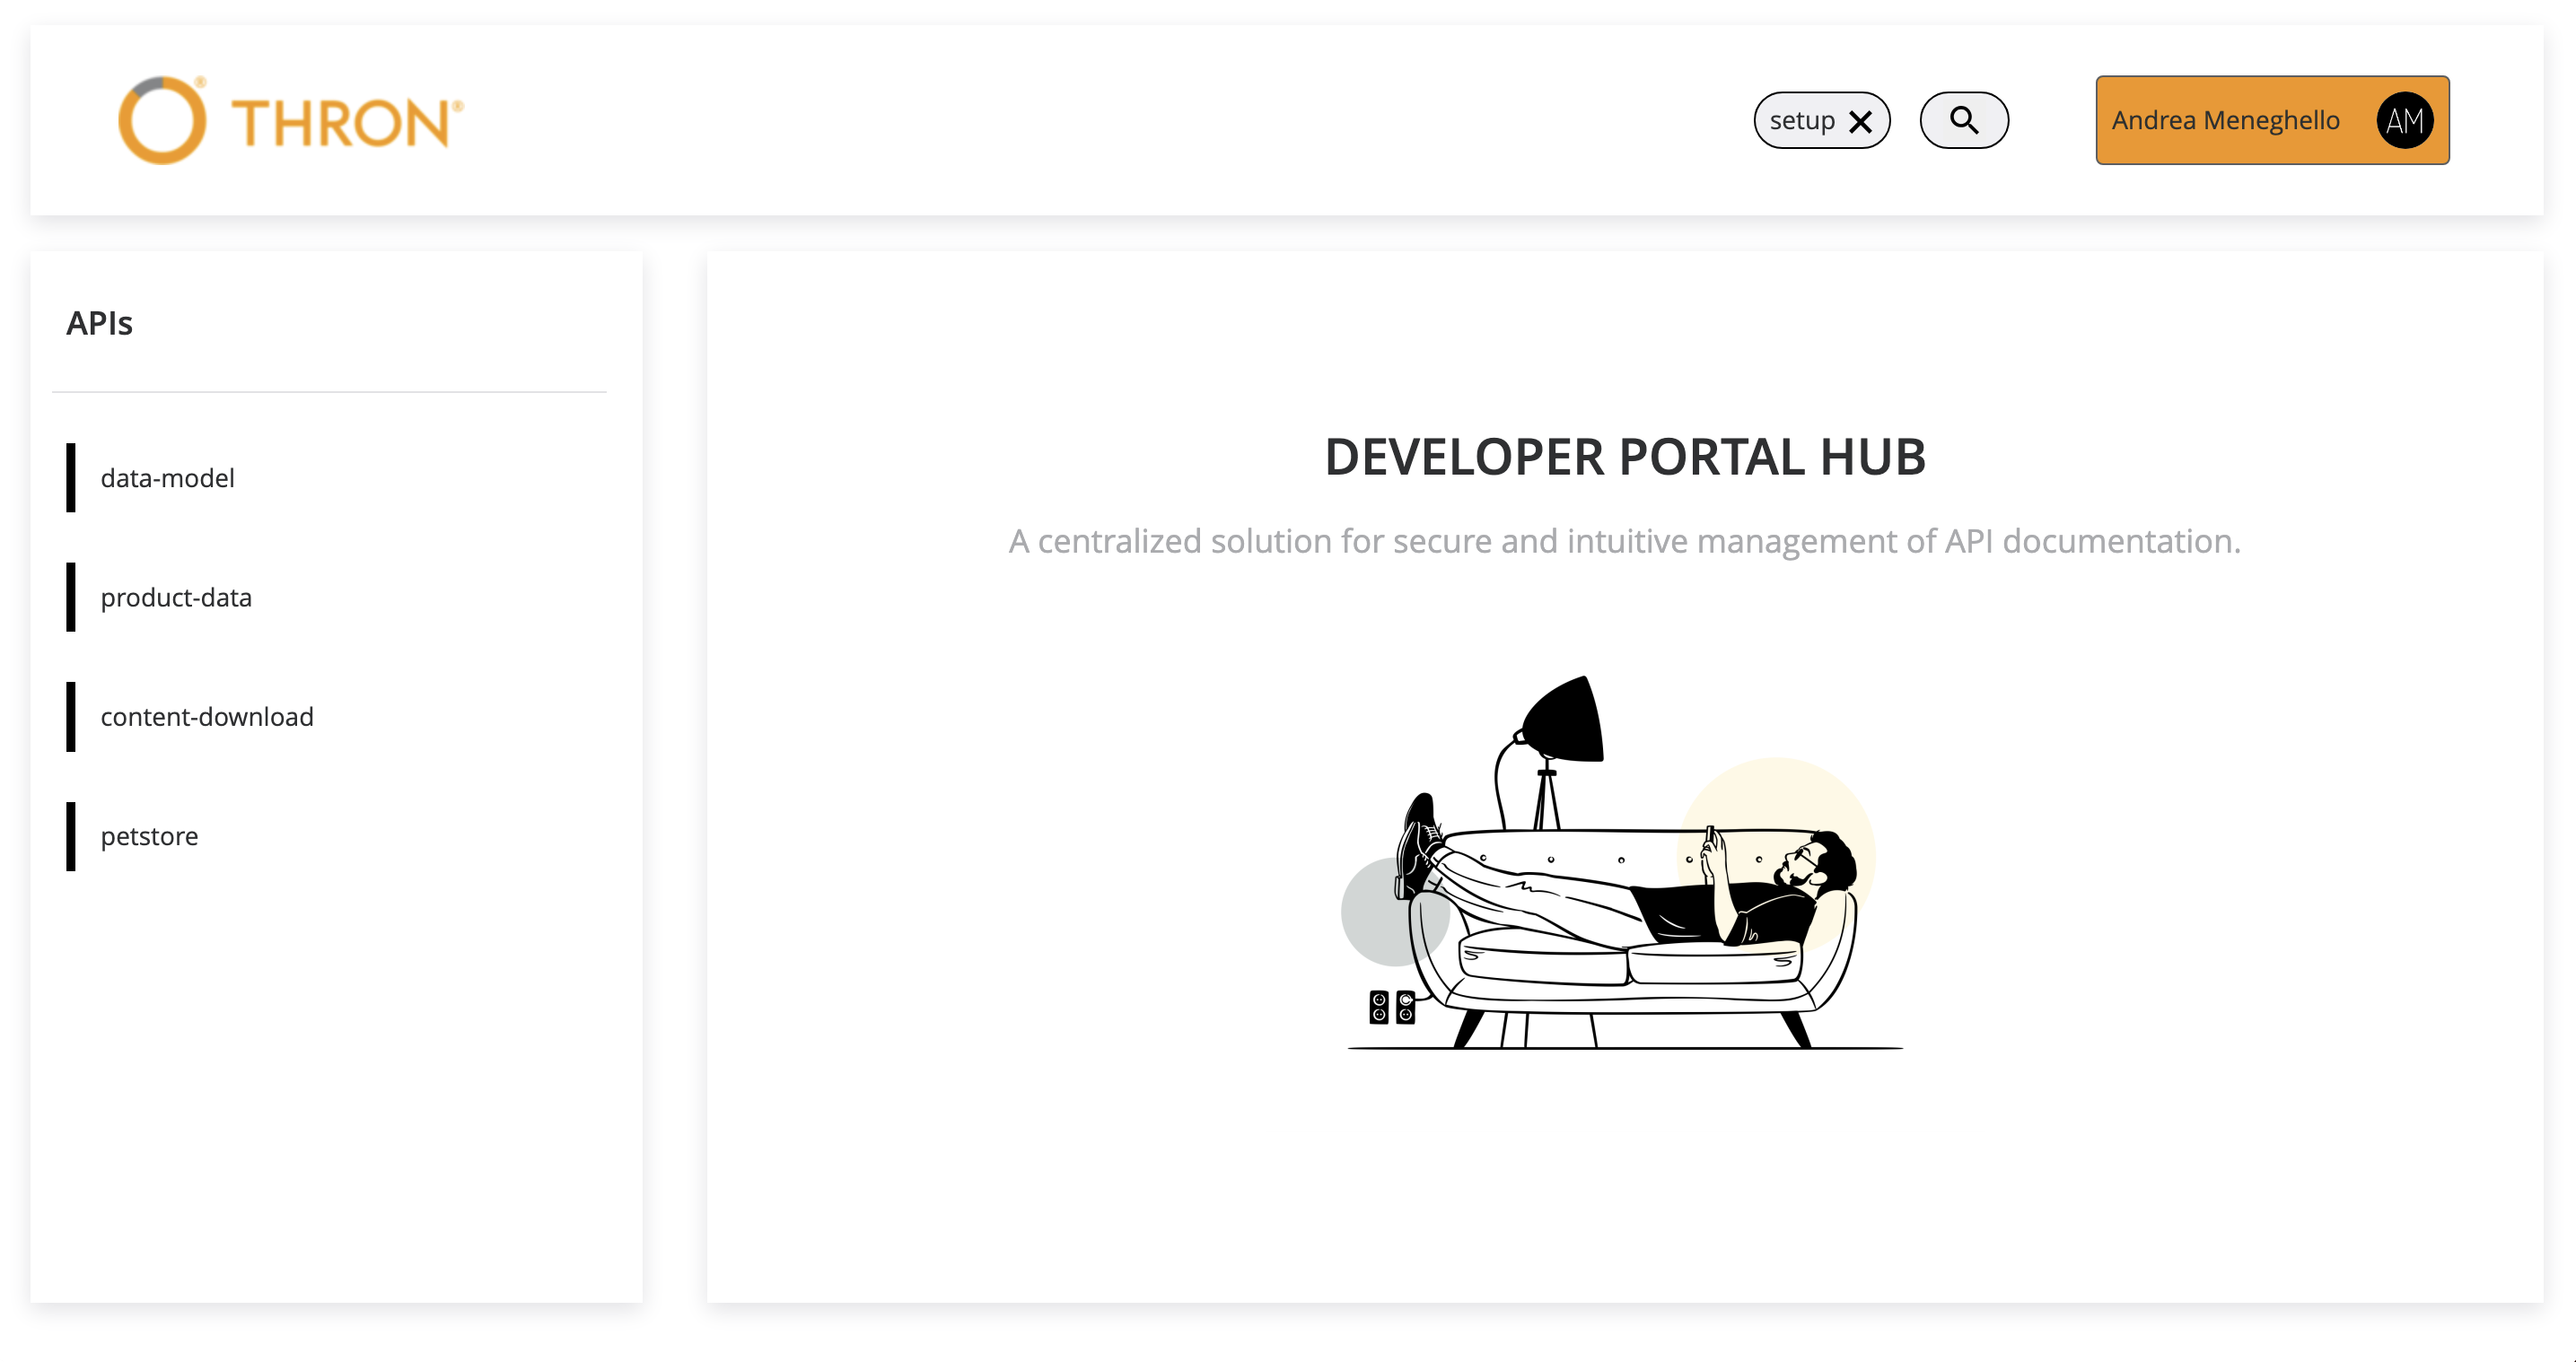
\includegraphics[width=0.6\textwidth, alt={Pagina principale dell'applicazione}]{images/frontend/HomeView.jpg}
  \caption{HomeView}\label{fig:home-view}
\end{figure}
\pagebreak

Come la pagina di login, anche la pagina principale è stata sviluppata con un \textit{design responsive} (in figura~\ref{fig:home-view-responsive}).
Come si vede dall'immagine si può notare che il menù laterale viene nascosto automaticamente e sarà accessibile cliccando l'apposito bottone a forma di \textit{hamburger}.

\begin{figure}[ht]
  \centering
  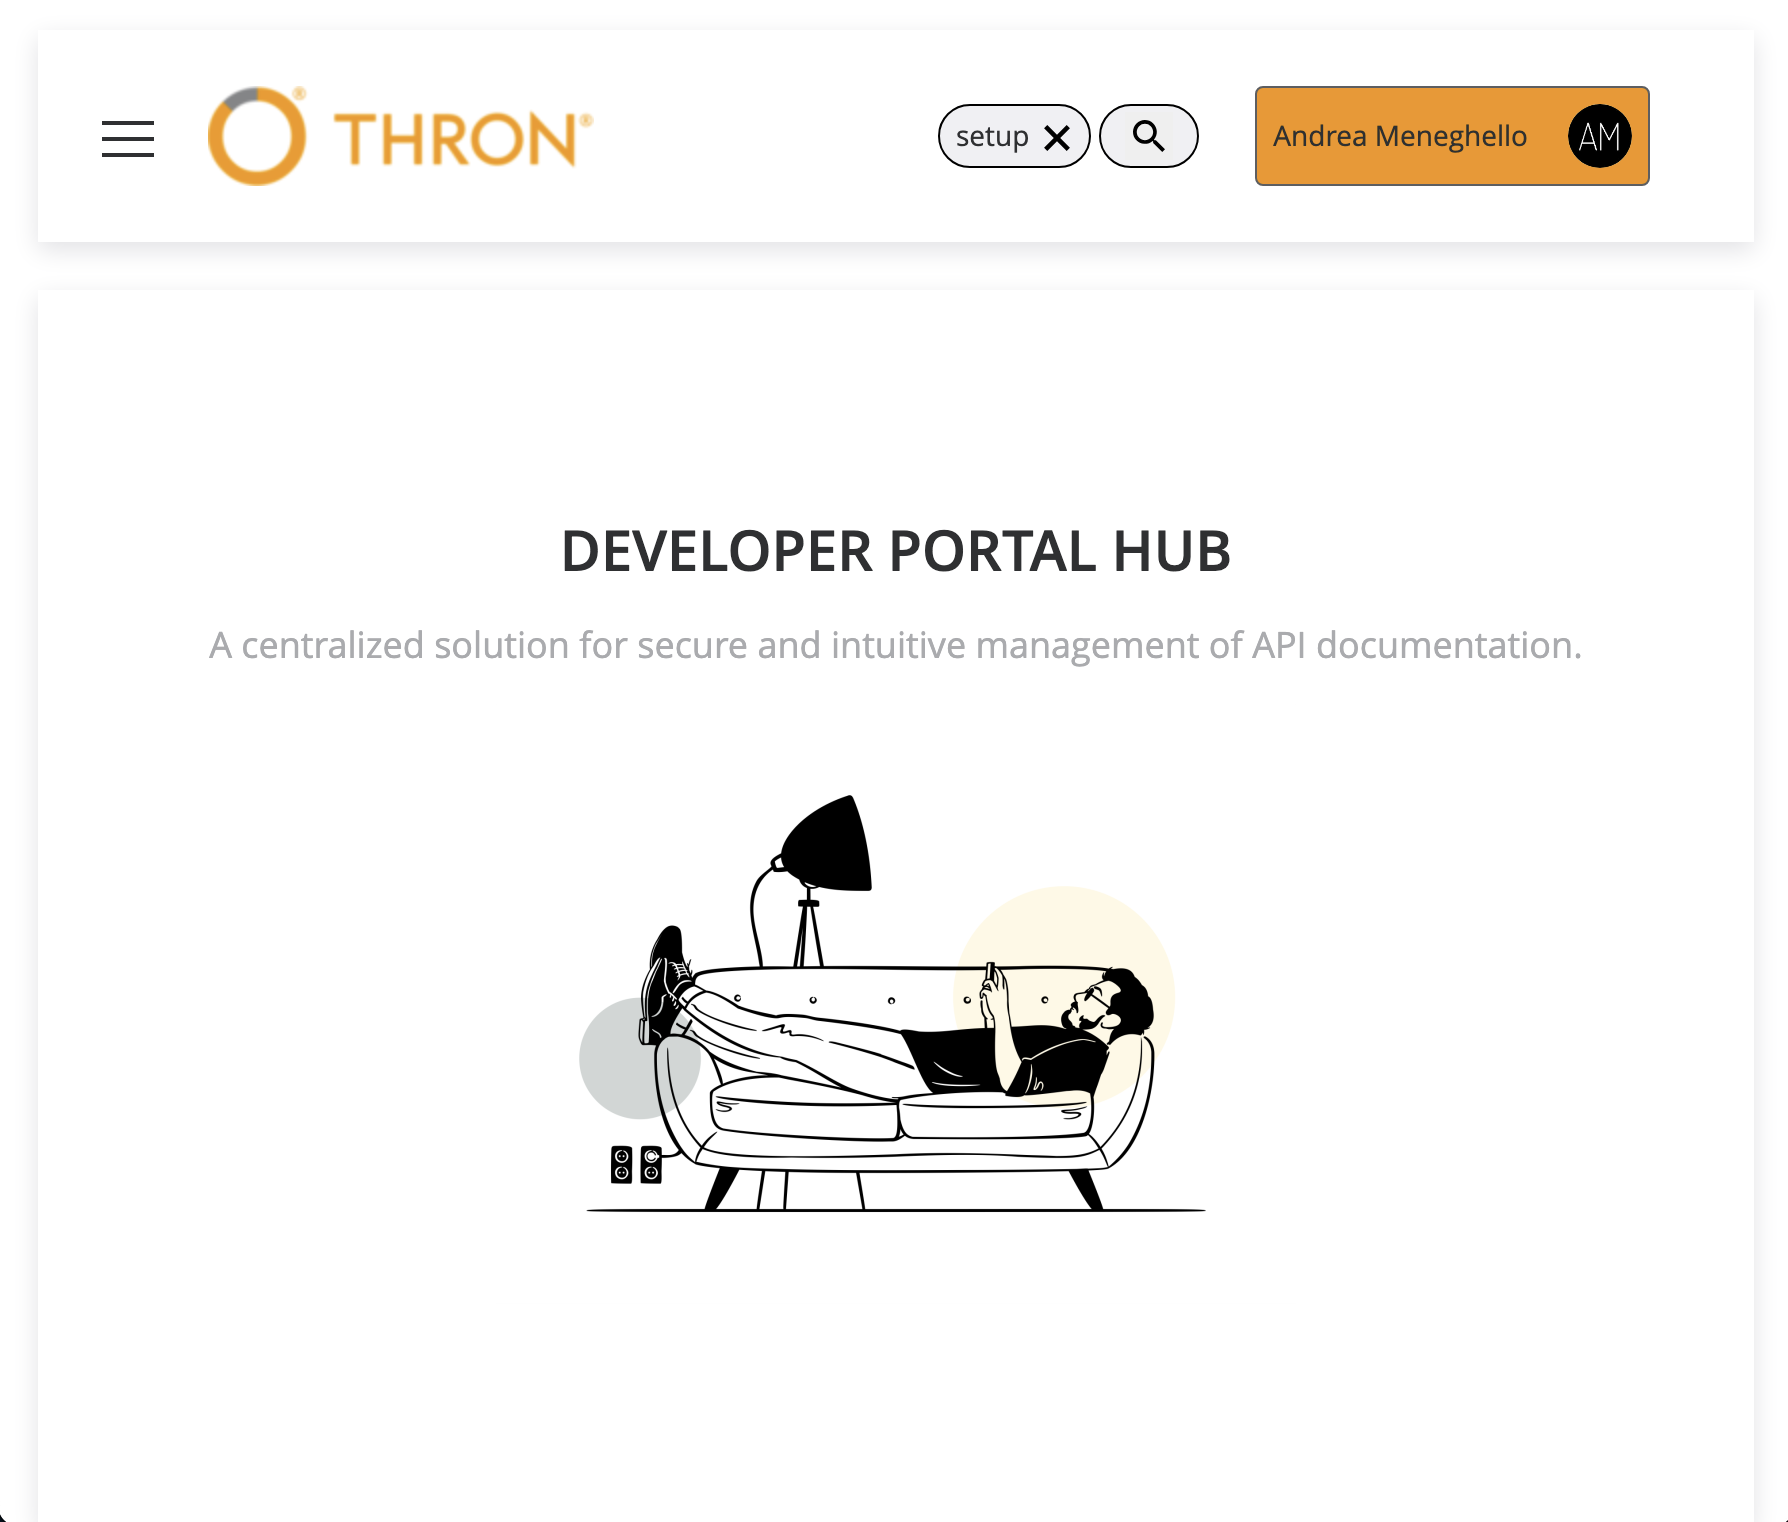
\includegraphics[width=0.6\textwidth, alt={Pagina principale responsive dell'applicazione}]{images/frontend/HomeViewRes.jpg}
  \caption{HomeView responsive}\label{fig:home-view-responsive}
\end{figure}


\paragraph{NotFoundView}\label{par:not-found-view}
Quando un utente tenta di accedere ad una pagina non esistente, verrà reindirizzato automaticamente alla pagina di errore 404 (in figura~\ref{fig:not-found-view}).
La pagina consiste in un messaggio di errore con un'immagine, dove viene informato l'utente che la pagina richiesta non esiste.
Per tornare alla \textit{HomeView} basterà cliccare sul bottone \textit{Home} e si potrà continuare la navigazione all'interno del portale.

\begin{figure}[ht]
  \centering
  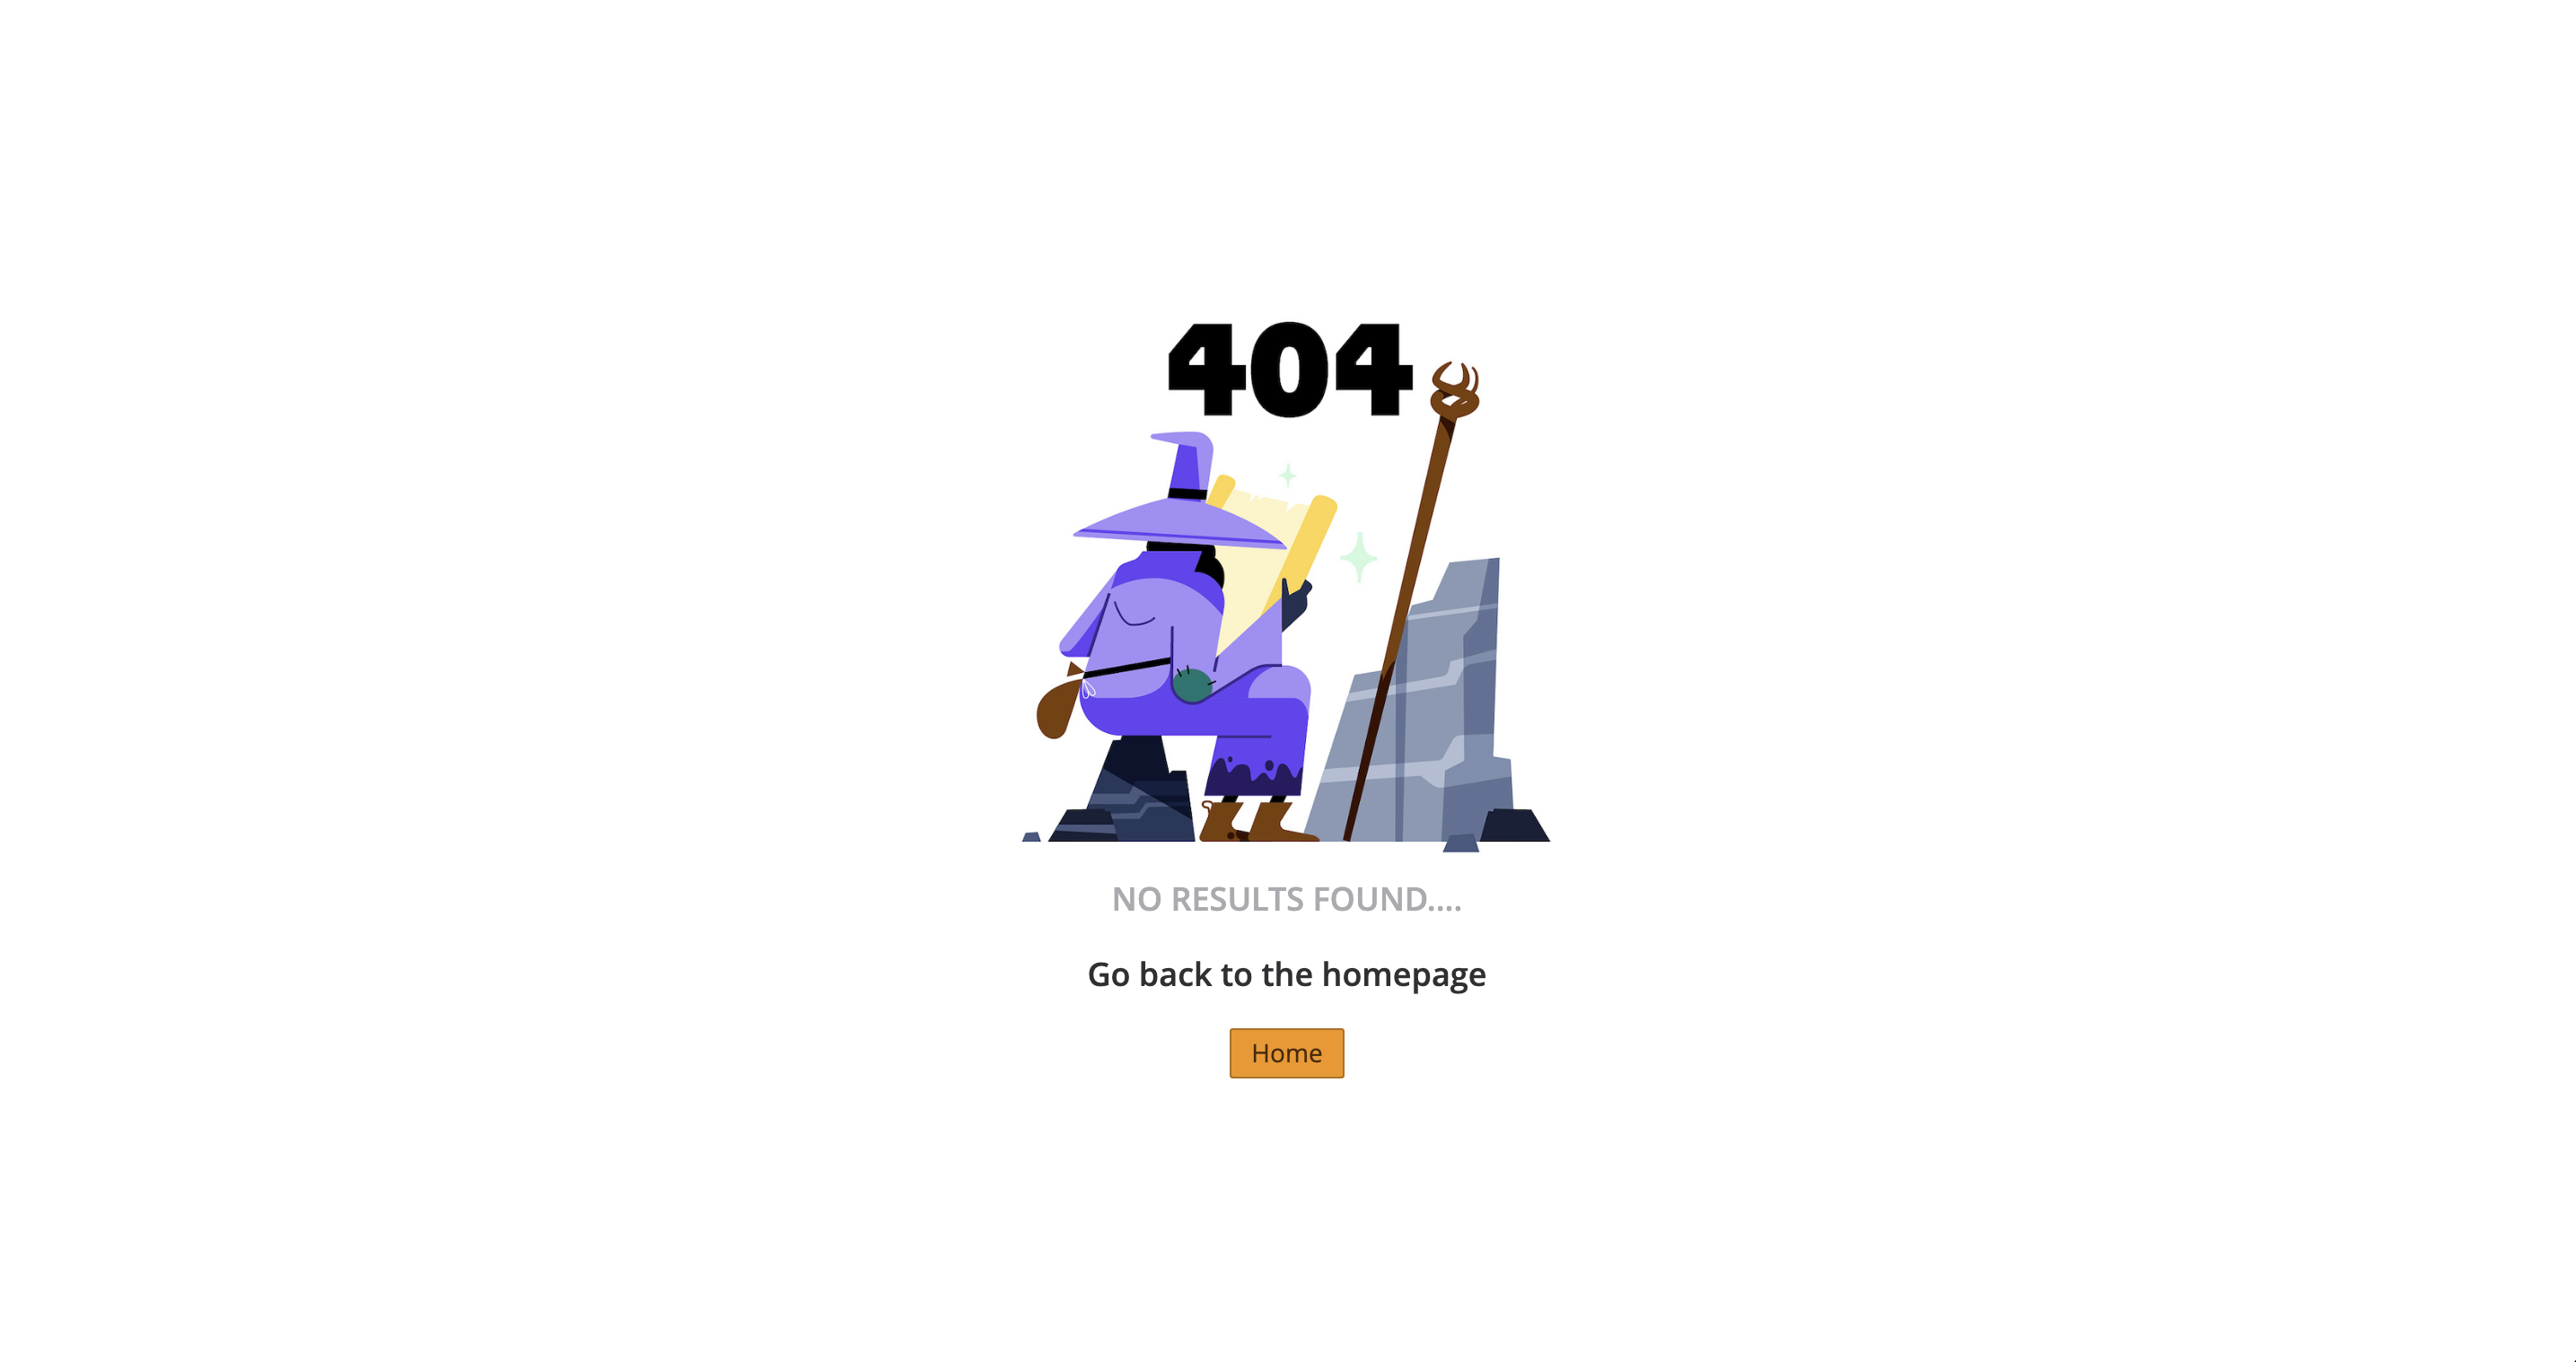
\includegraphics[width=0.6\textwidth, alt={Pagina di errore 404}]{images/frontend/NotFoundView.jpg}
  \caption{NotFoundView}\label{fig:not-found-view}
\end{figure}
\pagebreak
\subsubsection{Components}\label{subsubsec:components}

% Home
\paragraph{HeaderNav}\label{par:header-nav}
Il componente rapppresenta la barra di navigazione superiore dell'applicazione. Esso contiene il logo dell'applicazione, la \textit{chip} con il client-id
corrente, il bottone di ricerca e il \textit{popover} di logout. 
La barra viene visualizzata sempre una volta che l'utente ha effettuato il login.\\

\paragraph{MainContent}\label{par:main-content}
Il componente rappresenta il contenuto principale dell'applicazione. Esso infatti contiene la struttura per visualizzare i dettagli di ogni API (in figura~\ref{fig:main-content}), tramite l'aiuto 
della libreria \textit{Swagger UI}.
La struttura è la classica struttura di un documento Swagger, ovvero con una descrizione iniziale, la lista degli endpoint e infine la lista dei modelli.
I colori utilizzati sono uguali a quelli utilizzati in un comune Swagger, per dare un senso di familiarità all'utente ed è stata una richiesta avanzata dal team.
Nell'angolo destro è stato aggiunto un bottone per il download della documentazione, che verrà discusso in seguito.
\begin{figure}[ht]
  \centering
  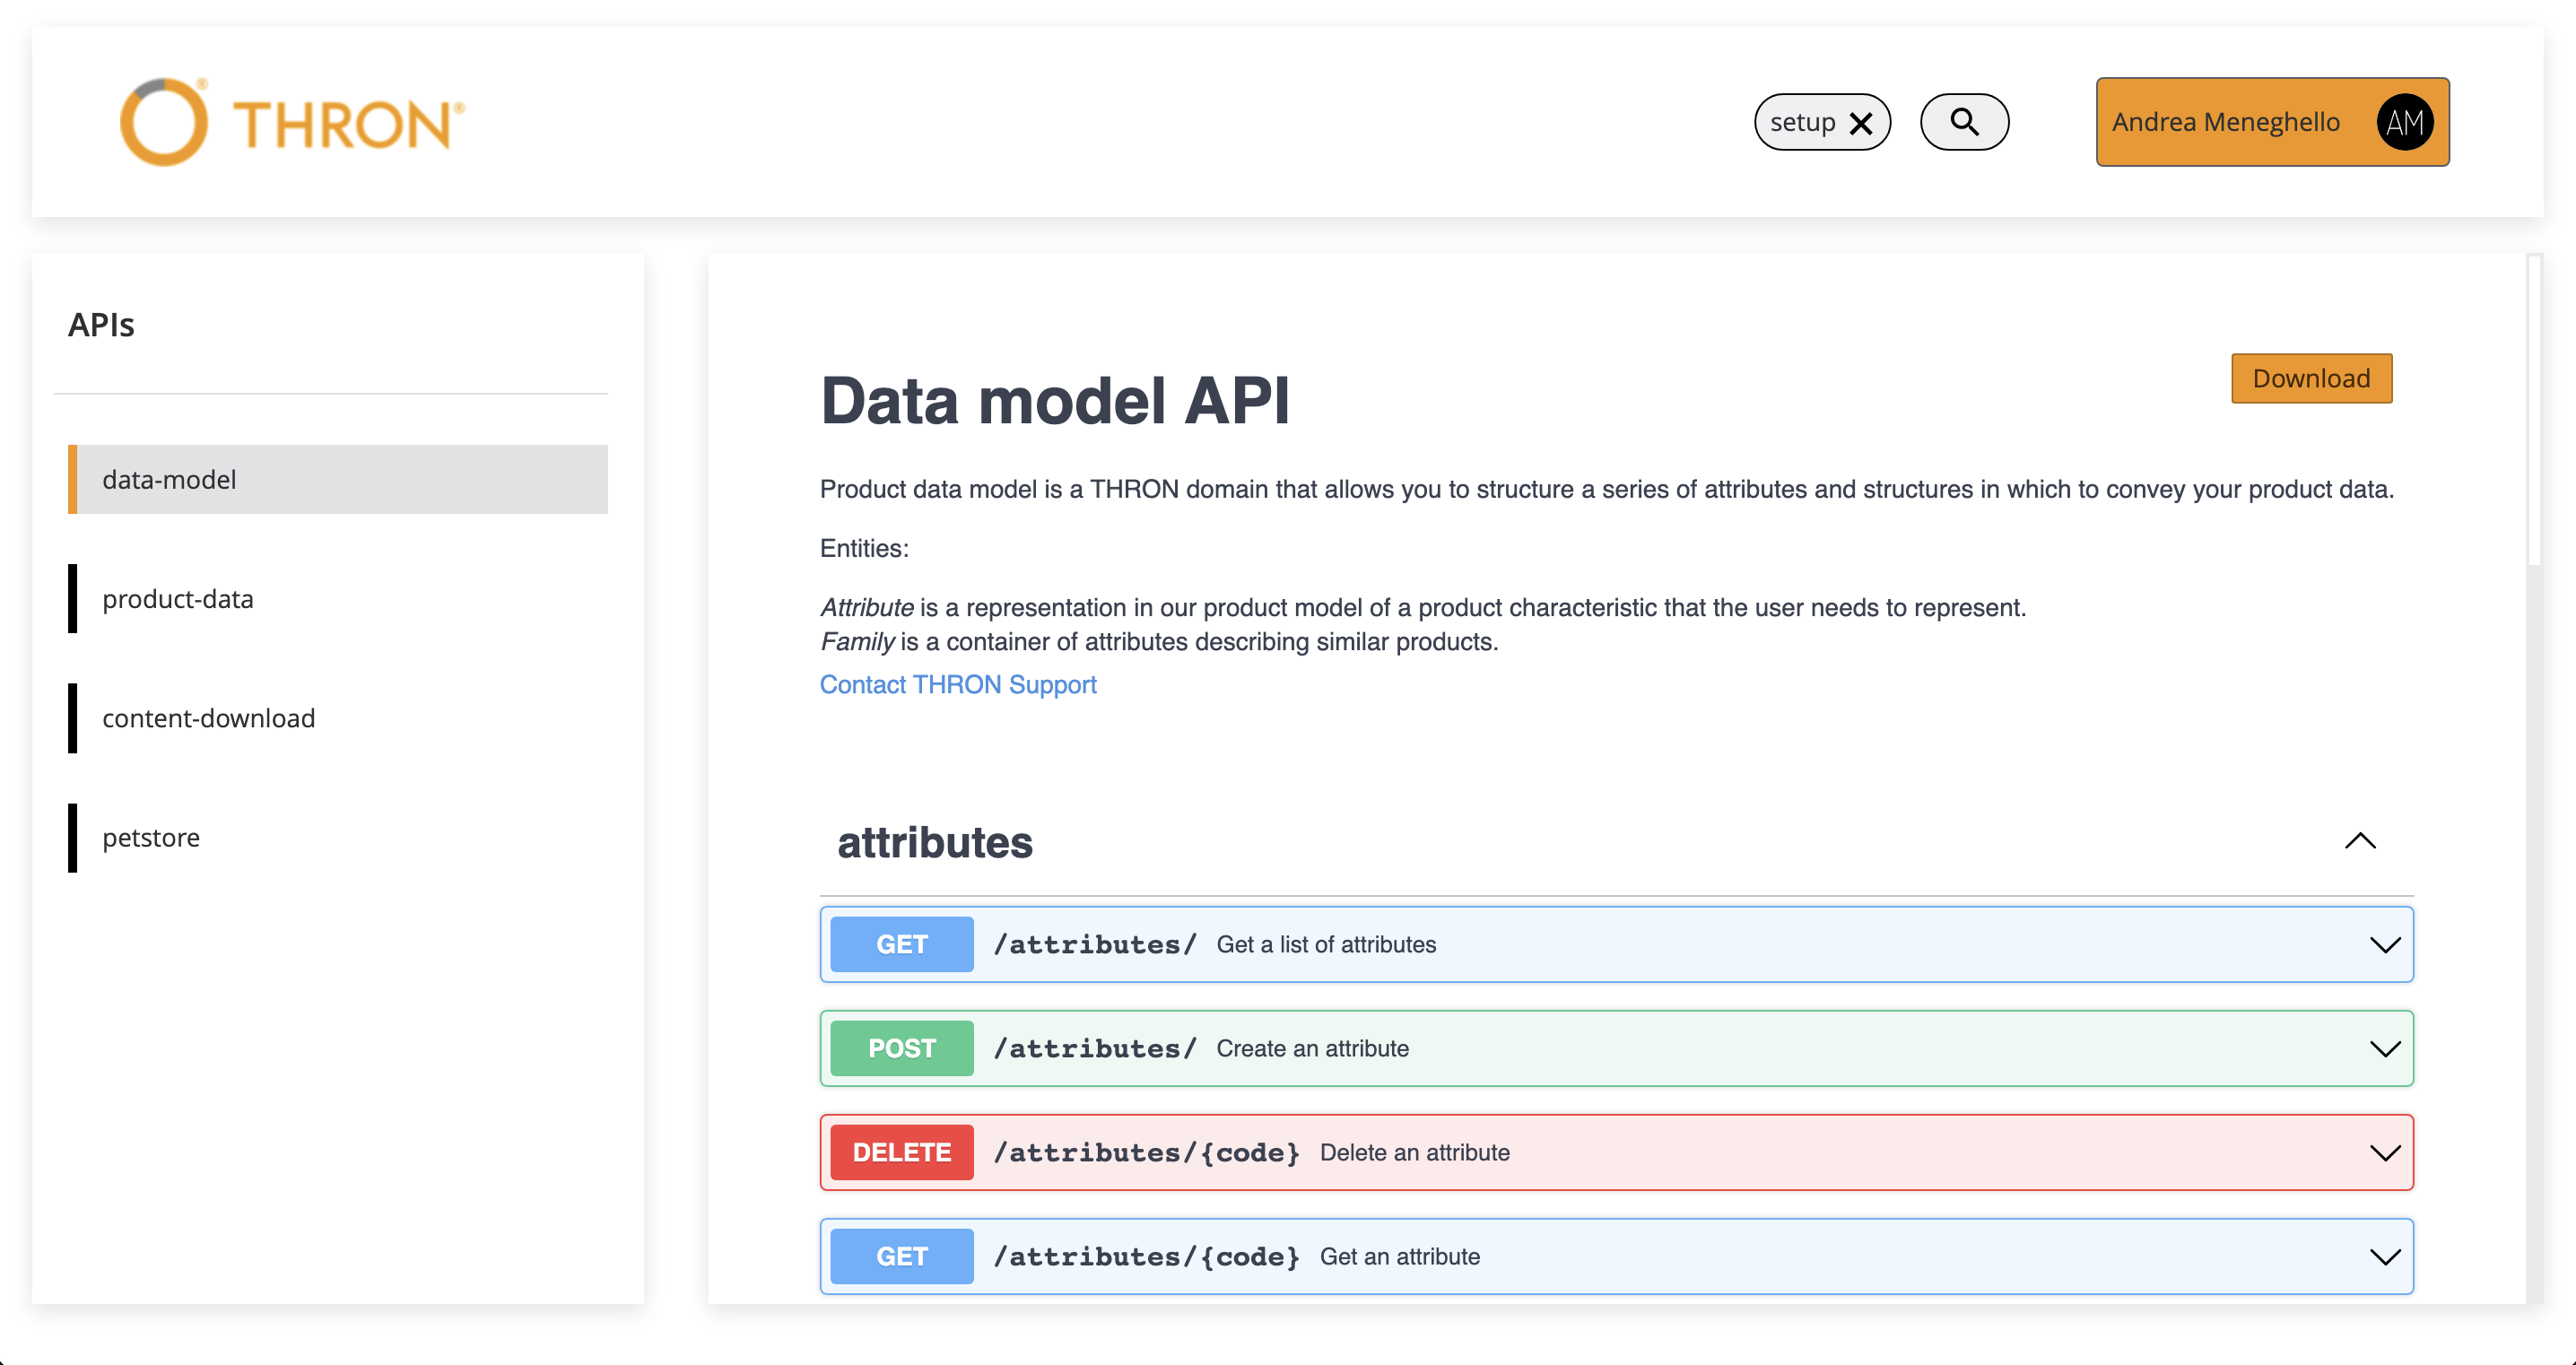
\includegraphics[width=0.6\textwidth, alt={Sezione per la visualizzazione dei dettagli di un API}]{images/frontend/DataModelView.jpg}
  \caption{MainContent}\label{fig:main-content}
\end{figure}
Cliccando su uno degli endpoint disponibili, ci sarà una sezione dedicata per la visualizzazione dei dettagli di esso (in figura~\ref{fig:try-it-out}).
I parametri e il \textit{Try it out} sono gestiti all'interno dello \textit{utils SwaggerUtils}, infatti il seguente componente comprende solo la definizione
della struttura.

\begin{figure}[ht]
  \centering
  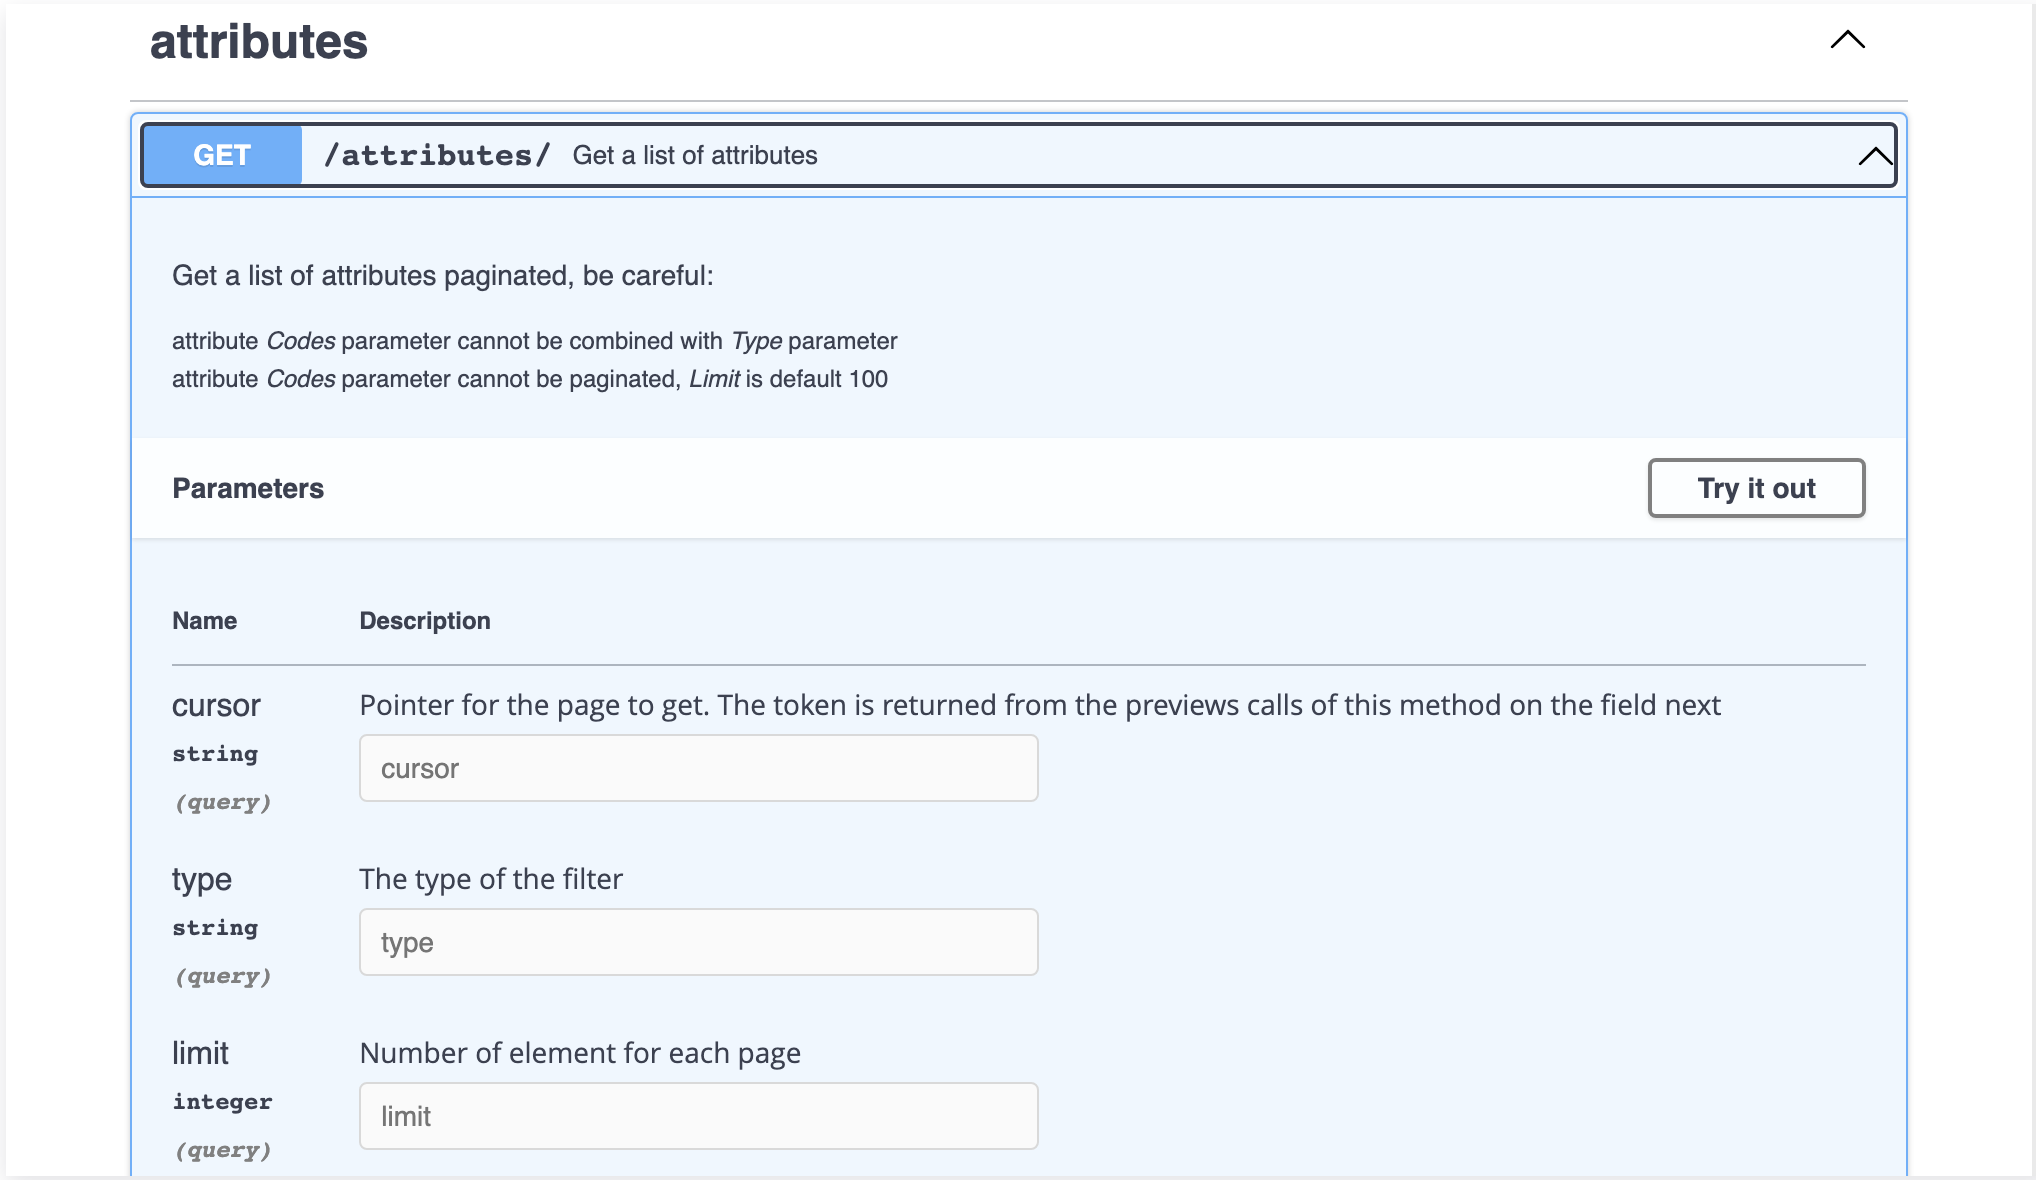
\includegraphics[width=0.6\textwidth, alt={Sezione try it out di un endpoint}]{images/frontend/TryItOut.jpg}
  \caption{Try it out}\label{fig:try-it-out}
\end{figure}

Inserendo i parametri e facendo quindi il \textit{try it out} verrà visualizzato il risultato della chiamata (in figura~\ref{fig:response}).

\begin{figure}[ht]
  \centering
  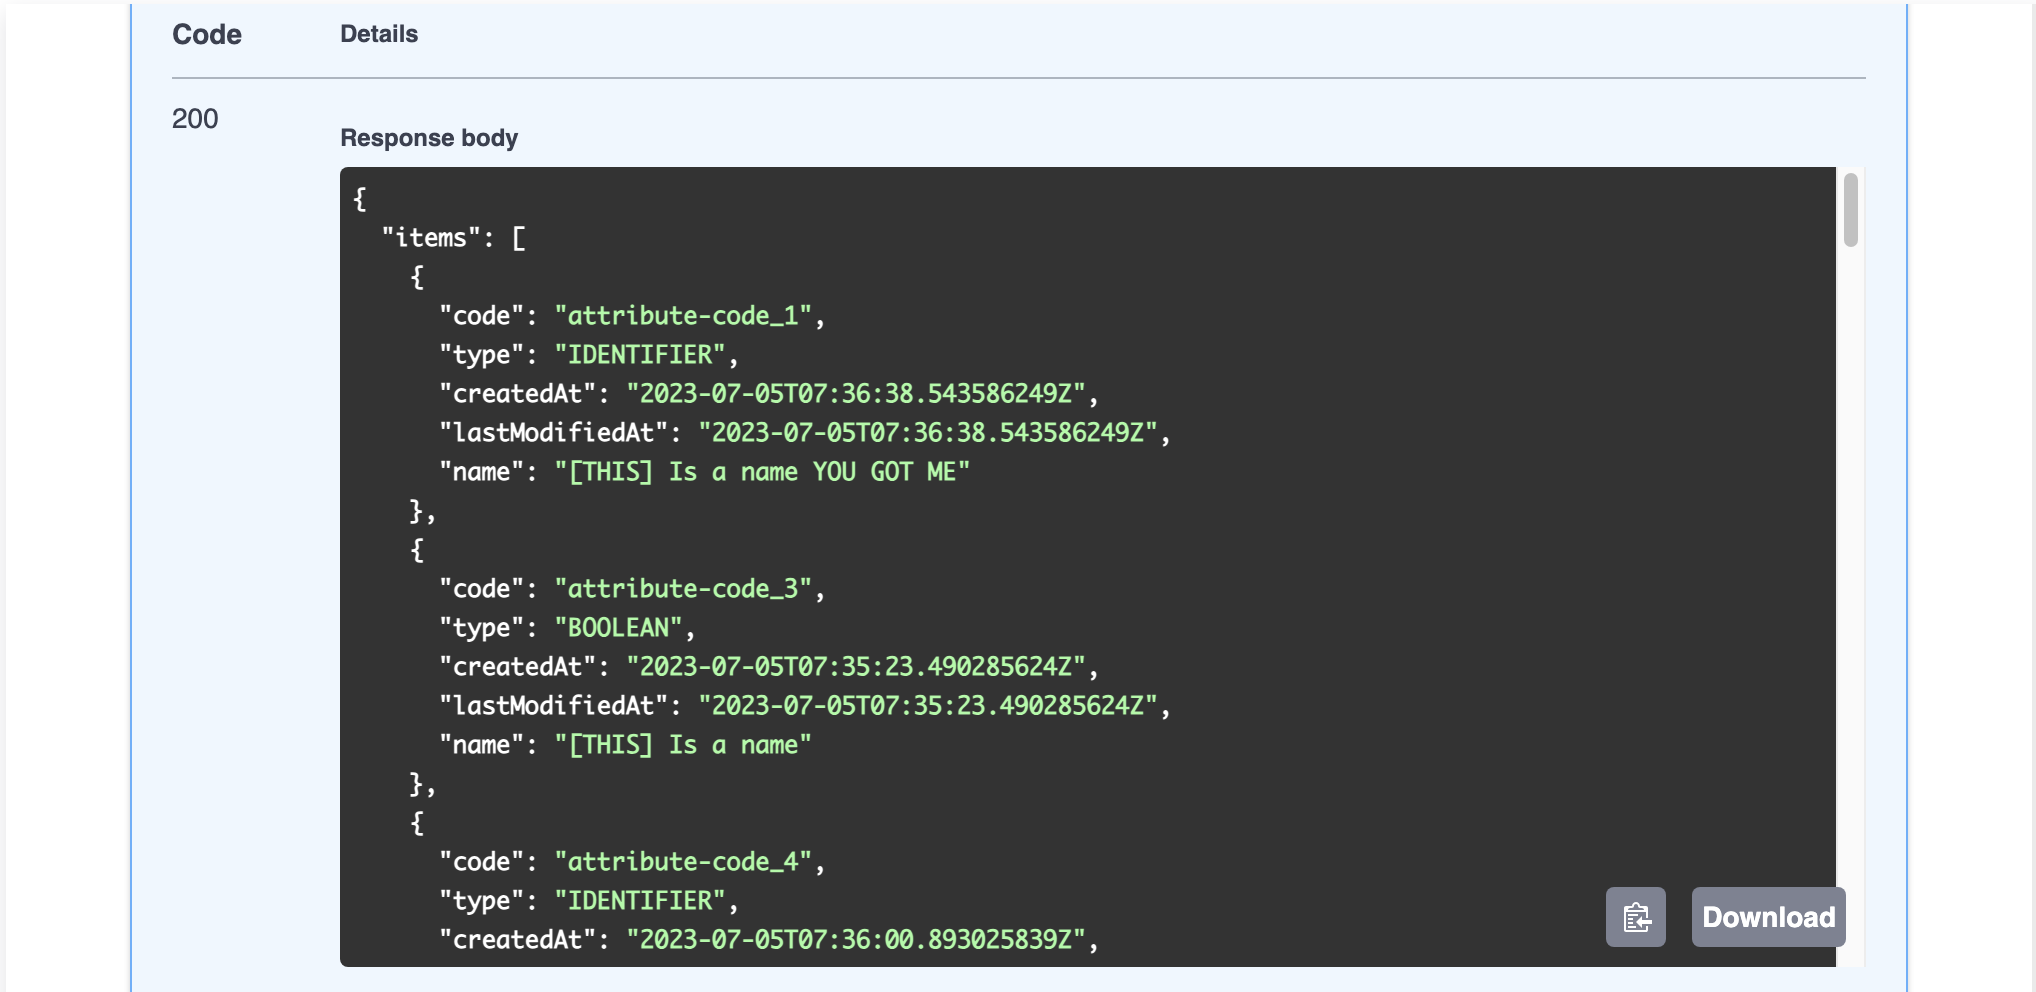
\includegraphics[width=0.6\textwidth, alt={Sezione per la visualizzazione della risposta di un endpoint}]{images/frontend/TryItOut3.jpg}
  \caption{Response}\label{fig:response}
\end{figure}

Inoltre al di sotto sarà presente anche una lista delle possibile risposte che l'endpoint può restituire (in figura~\ref{fig:response-list}).

\begin{figure}[ht]
  \centering
  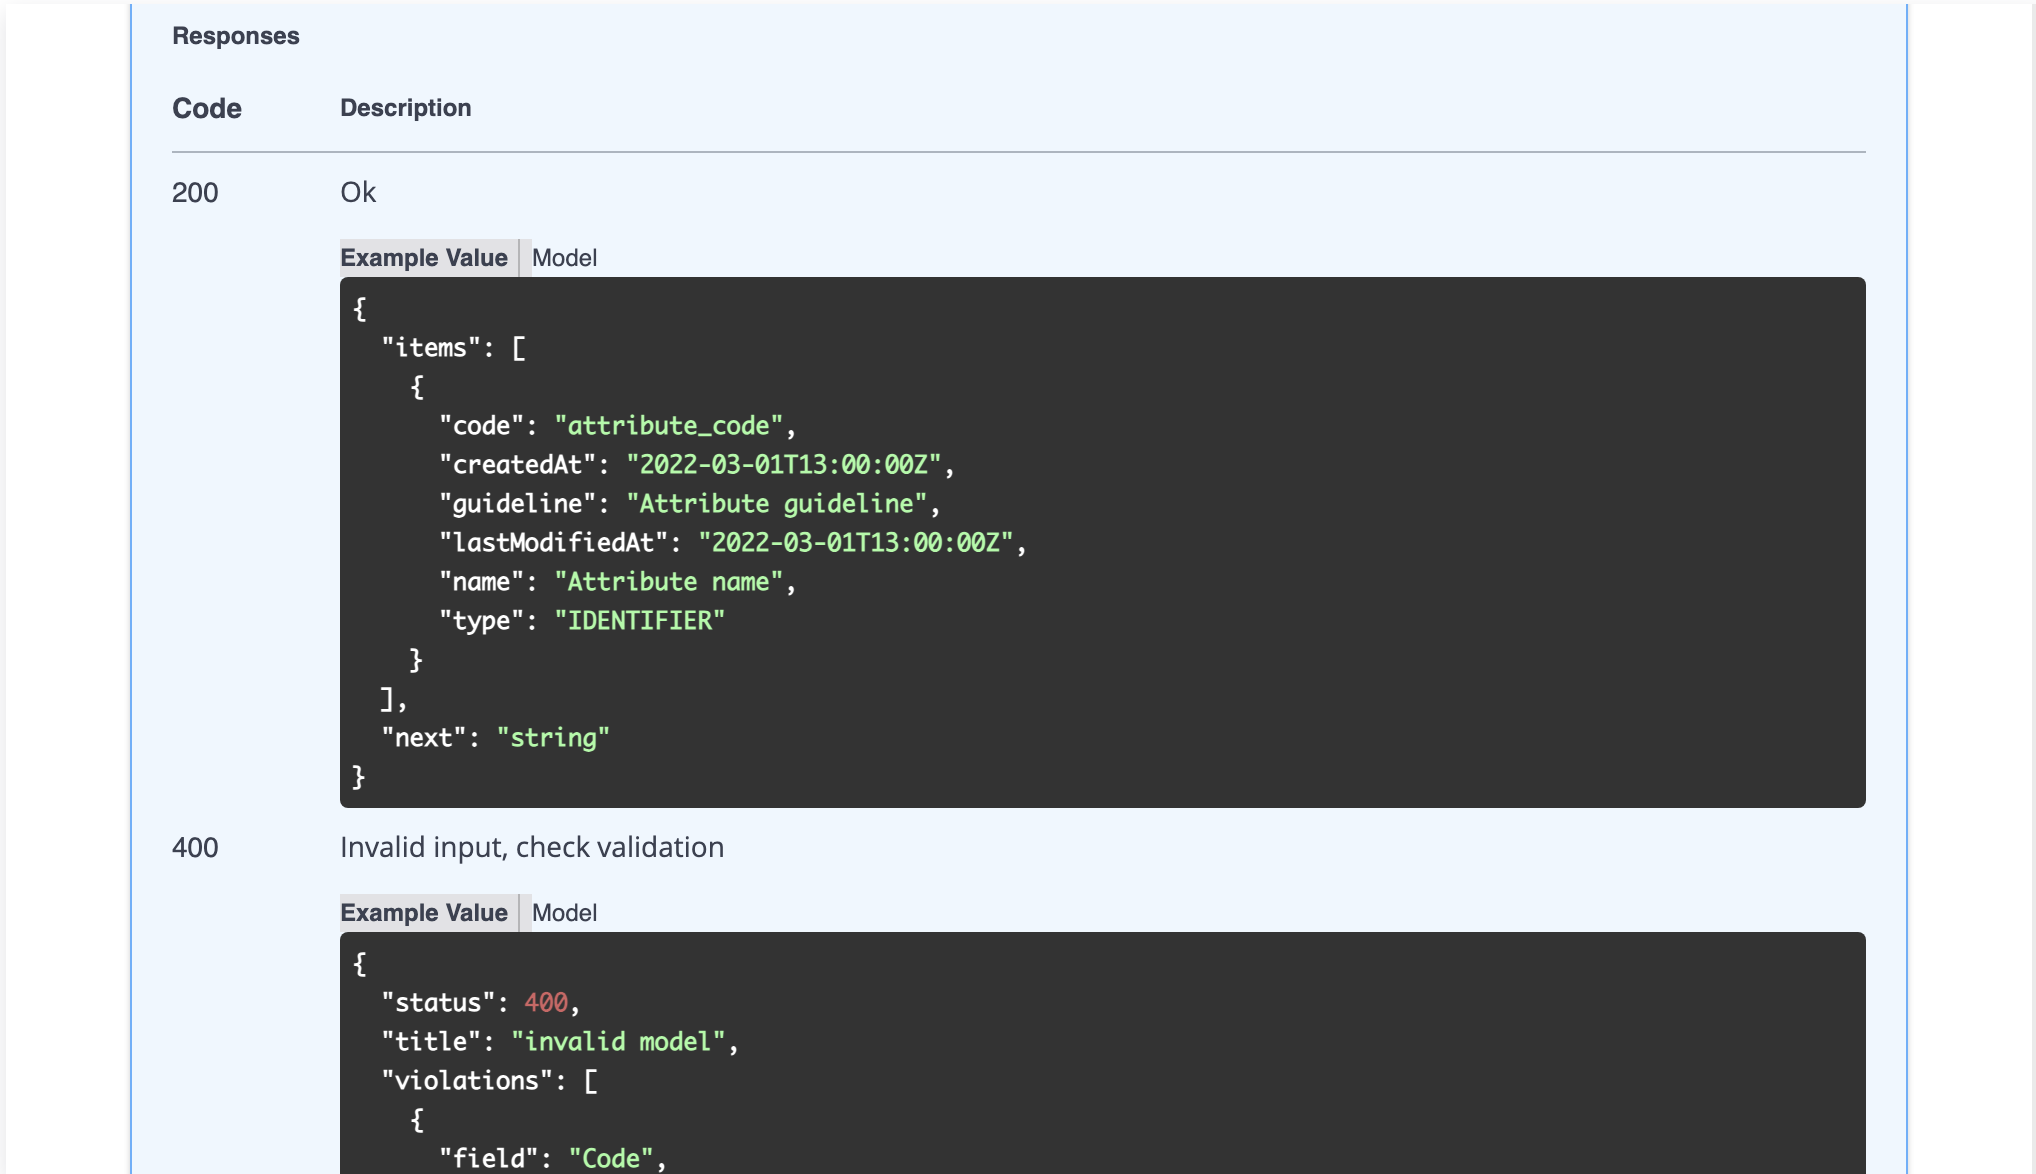
\includegraphics[width=0.6\textwidth, alt={Sezione per la visualizzazione delle possibili risposte di un endpoint}]{images/frontend/TryItOut4.jpg}
  \caption{Lista di risposte dell'endpoint}\label{fig:response-list}
\end{figure}

\pagebreak

Nel caso di chiamate con necessità del parametro \textit{client-id}, è stato gestito tramite l'\textit{utils SwaggerUtils} l'\textit{autofill} di esso.
Infatti, il campo verrà compilato con il \text-it{client-id} presente nella \textit{chip}, evitando che si inseriscano valori non presenti per 
quell'ambiente di sviluppo.
%scrivere di link

\paragraph{SideBar}\label{par:side-bar}
Il componente rappresenta la barra di navigazione laterale dell'applicazione. Esso contiene la lista di tutte le API disponibili nel portale.
Attraverso la barra sarà possibile navigare tra le varie API, andando a visualizzare i dettagli di ognuna di esse. 
Il componente è stato sviluppato utilizzando un design responsive, che permette di visualizzare il contenuto in maniera ottimale anche su spazi ridotti, 
infatti il menù andrà a nascondersi automaticamente e sarà accessibile cliccando l'apposito bottone a forma di \textit{hamburger}.\\


\paragraph{StartPage}\label{par:start-page}
% \gls{apig} è un portale che permette di consultare la documentazione delle API disponibili nel sistema.
Il componente rappresenta la pagina iniziale di benvenuto dell'applicazione ed è la prima schermata che l'utente visualizza dopo aver effettuato il login con successo.
Essa contiene il nome del portale, una breve descrizione e un'immagine. Per iniziare la navigazione nel portale, basterà usare la \textit{SideBar}.

\paragraph{SwaggerLoader}\label{par:swagger-loader}
Il componente rappresenta il loader di caricamento per il \textit{MainContent} (in figura~\ref{fig:swagger-loader}). 
Esso rappresenta un caricamento di stile \textit{skeleton}, ovvero un caricamento di contenuto che simula il contenuto finale, mentre questo viene caricato, attraverso un sfondo grigio dinamico.
Il componente ha la stessa struttura del \textit{MainContent}, quindi seguire lo stesso design responsive.
Il loader sarà visibile ogni volta che l'utente clicca su una delle API disponibili nella \textit{SideBar}, e scomparirà una volta che il contenuto sarà caricato correttamente.

\begin{figure}[ht]
  \centering
  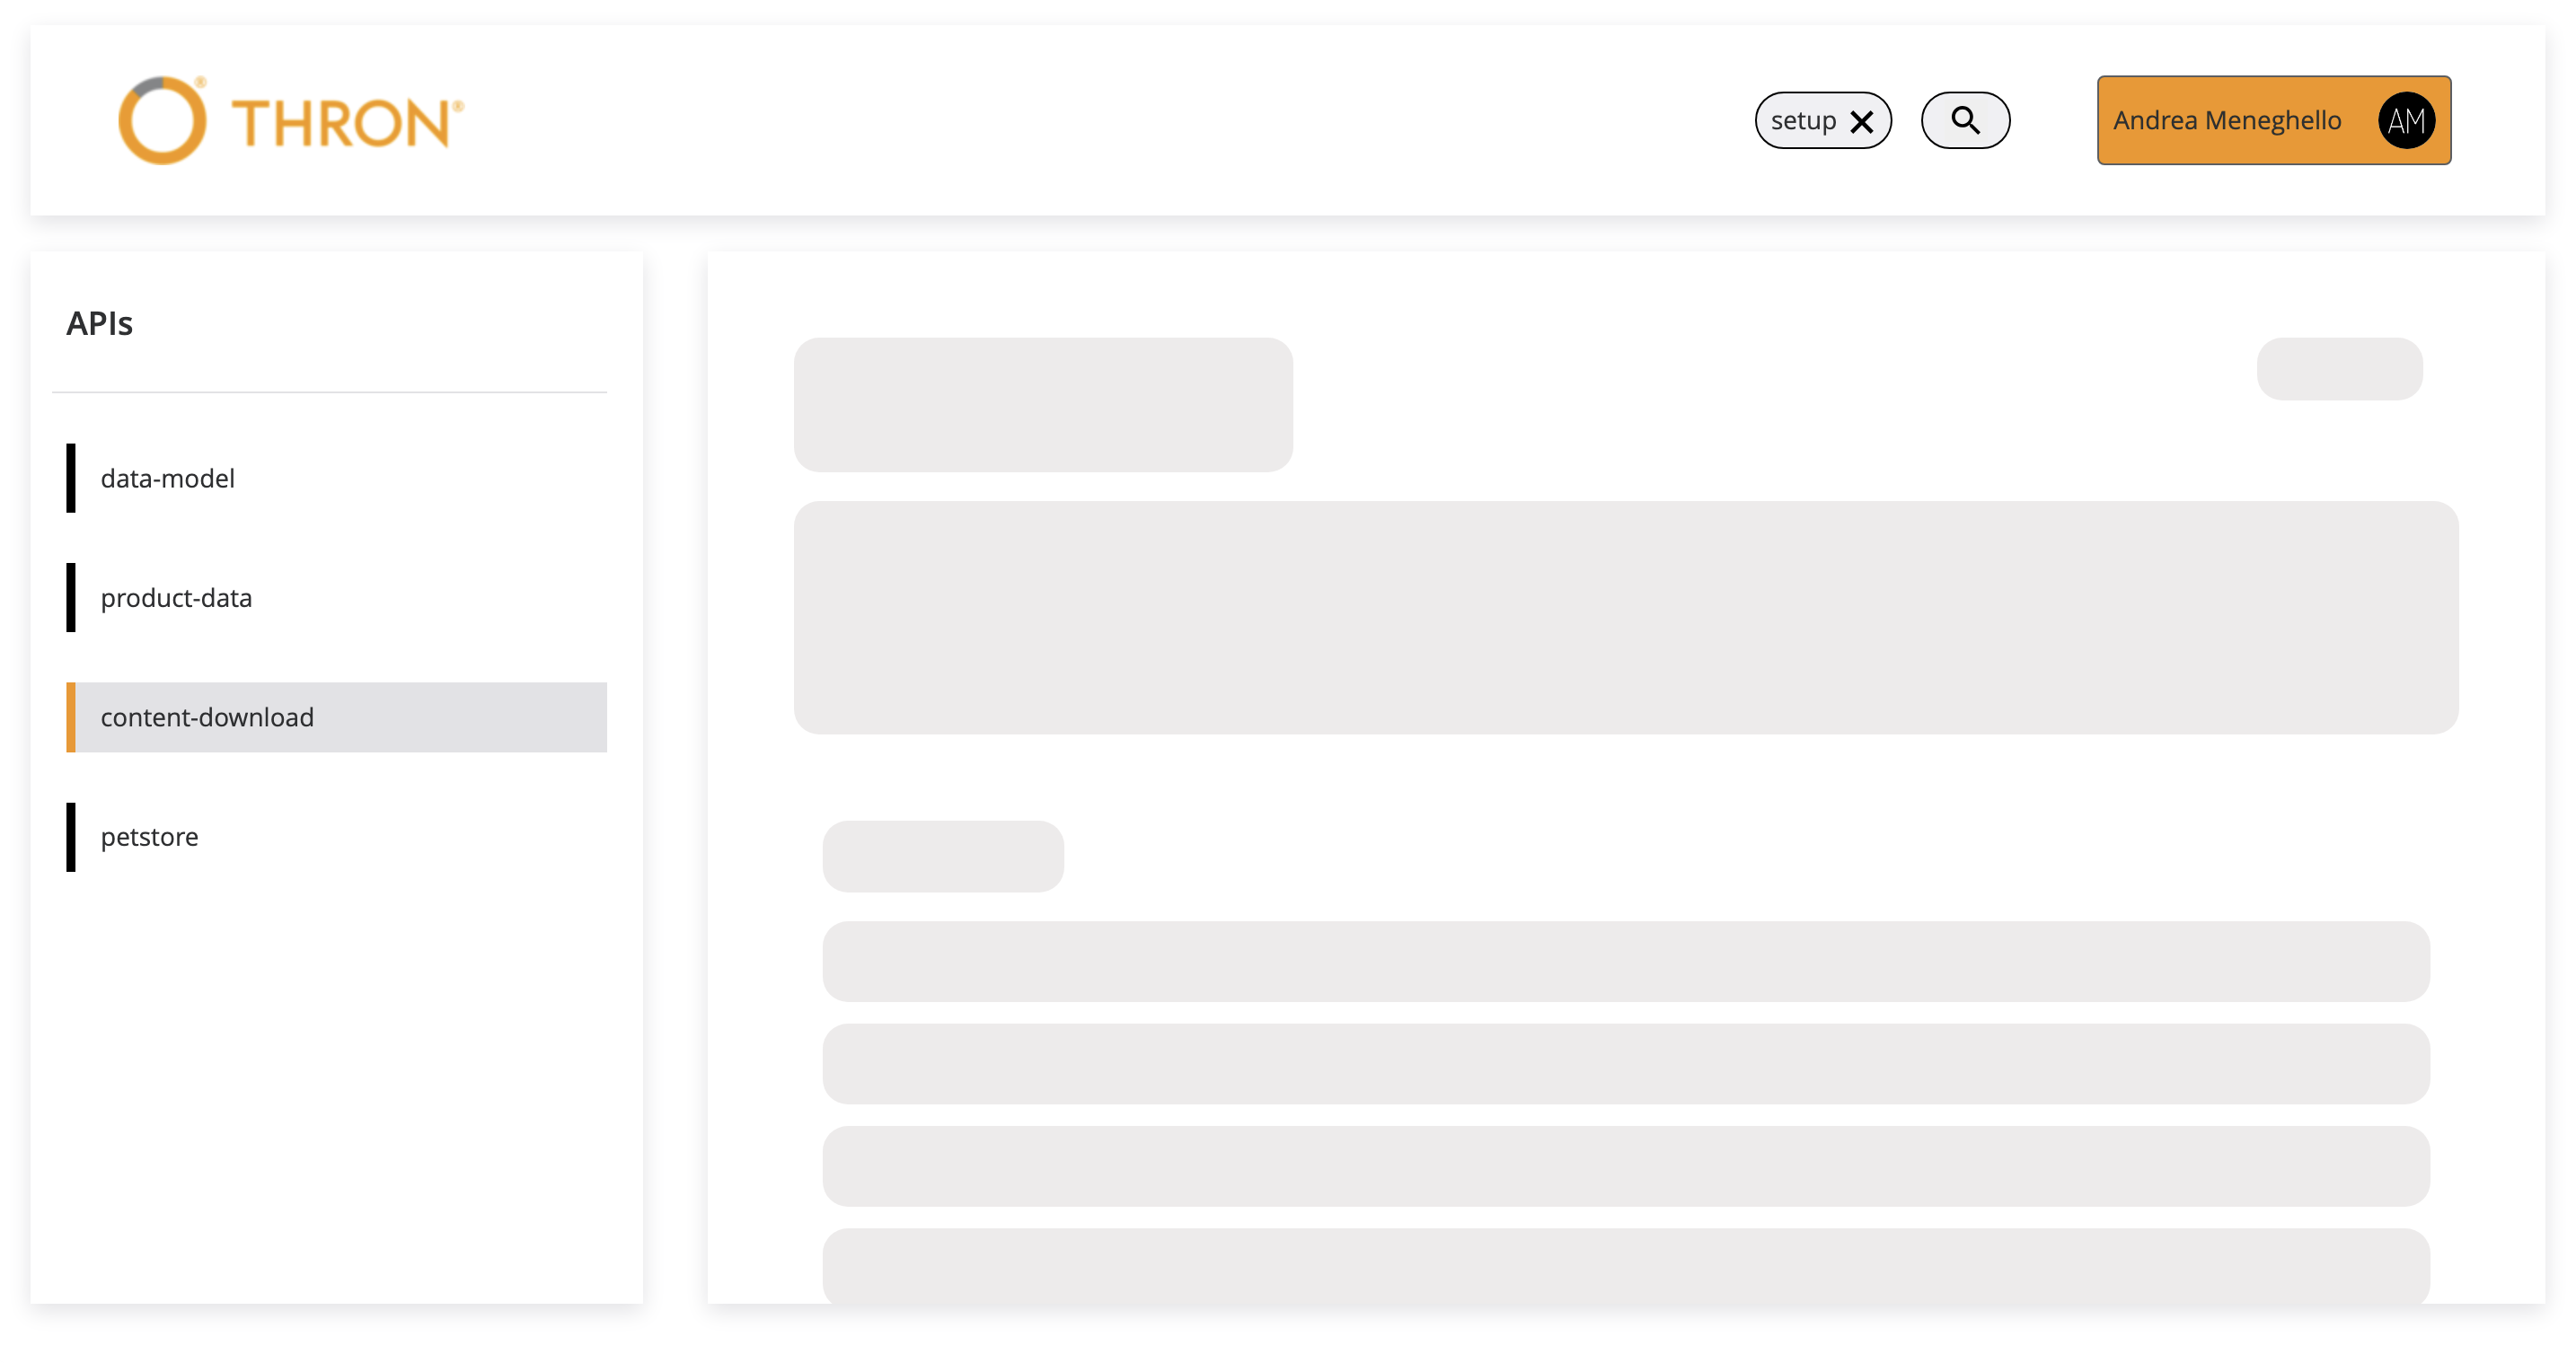
\includegraphics[width=0.6\textwidth, alt={Skeleton loader di caricamento per contenuto principale}]{images/frontend/SwaggerLoader.jpg}
  \caption{SwaggerLoader}\label{fig:swagger-loader}
\end{figure}

% \pagebreak
\paragraph{DownloadButton}\label{par:download-button}
Il componente rappresenta il bottone di download presente in ogni pagina di dettaglio dell'API specifica. Esso è stato sviluppato rispettando il \textit{design system}
aziendale, infatti non è un componente \textit{custom} creato da zero, ma è stato sviluppato utilizzando il componente \textit{Button} della libreria \textit{Components} THRON.
Il componente da la possibilità semplicemente di scegliere la grandezza, il testo del bottone e icone da visualizzare.
Il componente rende possibile all'utente di scaricare la documentazione dell'API in formato \textit{.yaml}, con un nome di file predefinito a seconda 
del servizio scaricato. Una volta cliccato, andrà ad aprire una finestra secondaria del browser, e il file verrà scaricato automaticamente.\\

\paragraph{LogoutButton}\label{par:logout-button}
Il componente rappresenta il bottone di logout presente nella barra di navigazione superiore dell'applicazione.
Esso è stato sviluppato rispettando il \textit{design system} aziendale, infatti utilizza la libreria \textit{Components} THRON.
Nello specifico è stato chiamato bottone per comodità, ma in realtà si tratta di un \textit{popover}, ovvero un componente a tendina che si apre
tramite l'\textit{hover} del mouse. Esso permette all'utente di effettuare il logout dal portale tramite un \textit{popup}, con successivo reindirizzamento
alla pagina di login.

%aggiungere foto hover

% Login
\paragraph{LoginButton}\label{par:login-button}
Il componente rappresenta il bottone di login presente nella pagina di login dell'applicazione. Esso è stato sviluppato rispettando il \textit{design system} aziendale.
Il seguente bottone aprirà un \textit{popup} dove sarà possibile inserire le credenziali (e-mail e password) per effettuare l'accesso tramite \textit{Microsoft} 365.
Una volta effettuato il login, l'utente verrà reindirizzato alla pagina principale del portale.

% Components
\paragraph{SearchButton}\label{par:search-button}
Il componente rappresenta il bottone di ricerca presente nella barra di navigazione superiore dell'applicazione.
Si tratta di un componente \textit{custom} creato da me, utilizzato per aprire la barra di ricerca globale del portale. 

\paragraph{SearchBar}\label{par:search-bar}
Il componente rappresenta la barra di ricerca globale dell'applicazione (in figura~\ref{fig:search-bar}). 
Essa consiste in una barra dove poter inserire il \textit{client-id} o il nome dell'\textit{API} da cercare,
con un'icona di ricerca a fianco. Per una migliore esperienza di ricerca, è necessario utilizzare il componente insieme al componente \textit{autocomplete} descritto in seguito.
Infatti i componenti insieme, costituiscono la ricerca all'interno del portale. Inoltre La \textit{SearchBar} è accessibile anche tramite tastiera,
infatti tramite il comando \textit{Ctrl + B} sarà possibile aprire la barra di ricerca.\\

\begin{figure}[ht]
  \centering
  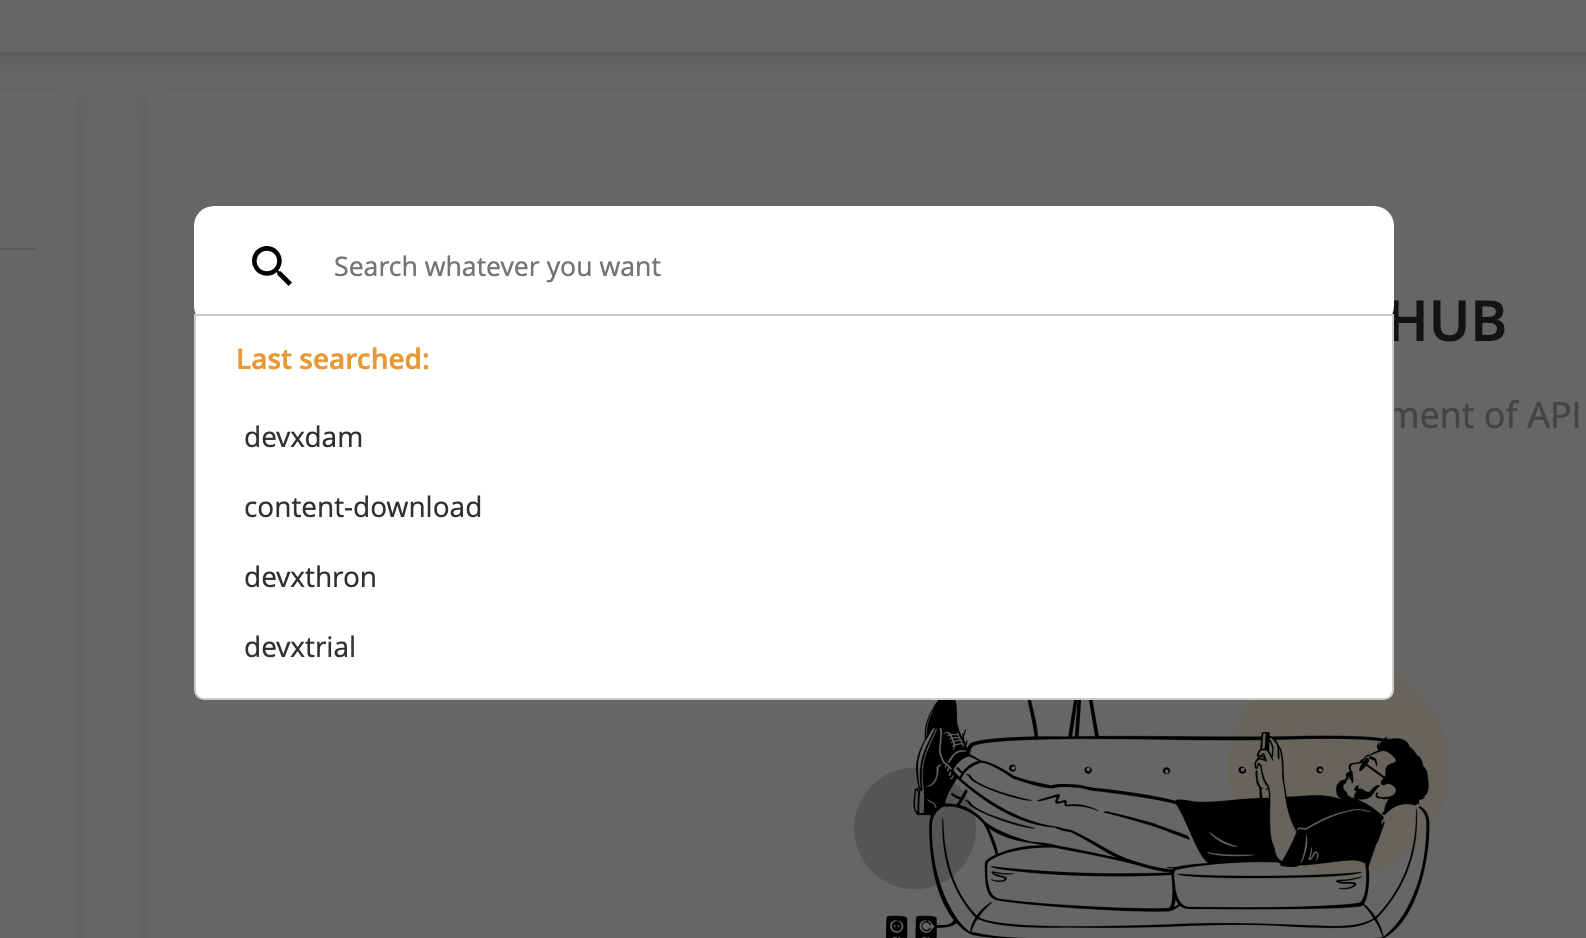
\includegraphics[width=0.6\textwidth, alt={Barra di ricerca globale dell'applicazione}]{images/frontend/SearchBar.jpg}
  \caption{SearchBar}\label{fig:search-bar}
\end{figure}

\paragraph{Autocomplete}\label{par:autocomplete}
Il componente rappresenta la lista di risultati visualizzata sotto la barra di ricerca dell'applicazione (in figura~\ref{fig:autocomplete}).
Essa consiste in una lista di suggerimenti dinamici che vengono visualizzati in base al testo inserito dall'utente. 
In caso il campo di ricerca della \textit{SearchBar} sia vuoto, verrà visualizzata se presente, la lista degli ultimi quattro termini cercati.
In caso contrario verrà visualizzata la lista dei suggerimenti con il numero di risultati trovati per ogni lista e il nome della lista.
Nel caso in cui la ricerca non abbia prodotto risultati, verrà visualizzato un messaggio di errore, gestito tramite il componente \textit{SnackBar} descritto in seguito.
La logica della ricerca, è completamente sviluppata lato \textit{backend} per estrapolare il componente di ricerca e renderlo riutilizzabile in altri progetti.
Essendo un componente \textit{custom}, ho aggiunto la possibilità di navigare il menù e selezionare un suggerimento tramite tastiera, funzionalità 
obbligatoria per rendere la ricerca accessibile anche a persone con disabilità.\\
Dopo aver selezionato un suggerimento, verrà aperta la pagina di dettaglio dell'API selezionata se l'utente ha scelto un'API, altrimenti verrà impostato il client-id corrente e la Chip verrà aggiornata.
Il componente infine, supporta più liste di elementi per la ricerca globale, non solo due, infatti sarà possibile anche avere un numero vario liste di elementi in cui effettuare
la ricerca globale. 

\begin{figure}[ht]
  \centering
  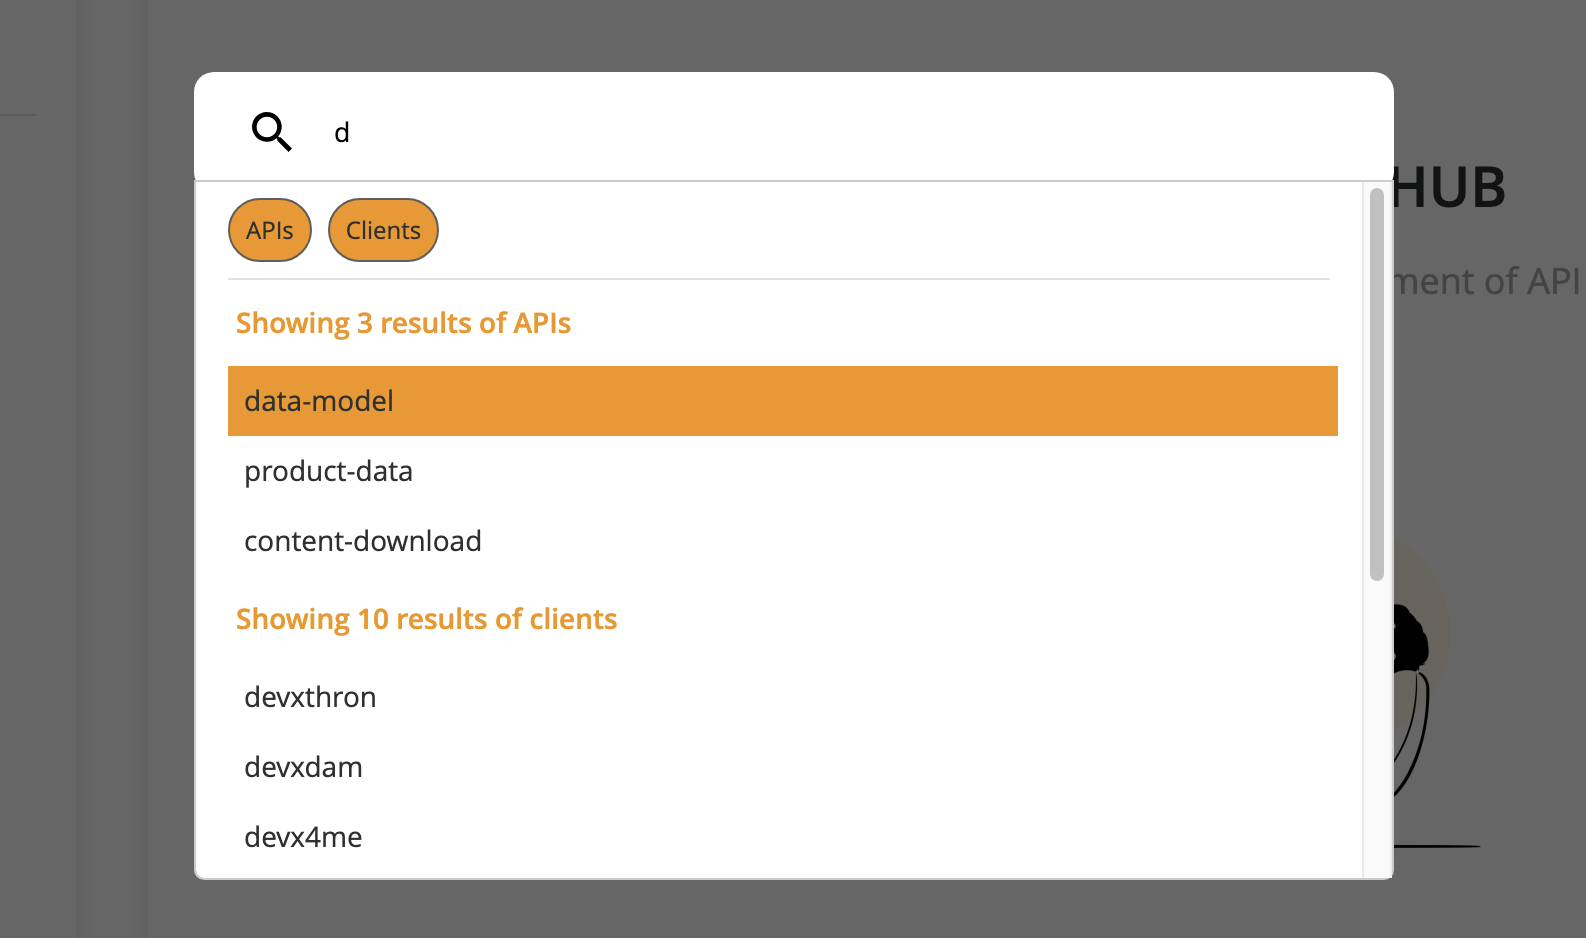
\includegraphics[width=0.6\textwidth, alt={Componente che si occupa della lista dinamica di risultati}]{images/frontend/SearchBar2.jpg}
  \caption{Autocomplete}\label{fig:autocomplete}
\end{figure}

\paragraph{Chip}\label{par:chip}
Il componente rappresenta la \textit{chip} situata nella barra di navigazione superiore dell'applicazione (in figura~\ref{fig:chip}).
Essa è utile a visualizzare il \textit{client-id} corrente, ovvero il \textit{client-id} che l'utente ha selezionato tramite la barra di ricerca globale.
In caso l'utente non abbia selezionato ancora nessun \textit{client-id}, verrà visualizzato il \textit{client-id} di default dell'ambiente di sviluppo.
Inoltre è possibile resettare il \textit{client-id} corrente, cliccando sull'icona di reset a forma di \textit{X}, riportandolo al valore di default.
In caso il \textit{client-id} fosse già al valore di default, verrà visualizzato un messaggio di errore tramite il componente \textit{SnackBar} descritto in seguito.

\begin{figure}[ht]
  \centering
  
\includegraphics[width=0.3\textwidth, alt={Chip contenente il client id corrente}]{images/frontend/Chip.jpg}
  \caption{Chip}\label{fig:chip}
\end{figure}


\paragraph{Filter}\label{par:filter}
Il componente rappresenta il bottone per filtrare la lista dei risultati della ricerca, all'interno del componente \textit{Autocomplete}.
Quando il bottone viene cliccato, lo sfondo risulta bianco e verrà visivamente nascosta la lista corrispondente al filtro cliccato.
Cliccando di nuovo sullo stesso filtro, il bottone tornerà arancione e verrà  mostrata la lista corrispondente al filtro cliccato.


\paragraph{OptionList}\label{par:option-list}
Il componente rappresenta la lista di opzioni generiche, visualizzate all'interno della SideBar. Nel mio progetto, è stata utilizzata per visualizzare la lista
di tutte le \textit{API} disponibili nel sistema. 

\paragraph{OptionListItem}\label{par:option-list-item}
Il componente rappresenta un singolo elemento della lista di opzioni generiche, visualizzate all'interno della SideBar. Nel mio progetto, un'\textit{item} rappresenta una singola \textit{API}.
Andando a cliccare un'opzione, verrà aperta la pagina di dettaglio dell'\textit{API} selezionata.

\paragraph{SnackBar}\label{par:snack-bar}
Il componente rappresenta la \textit{snack-bar} dell'applicazione usata per la visualizzazione di messaggi di errore o di successo (in figura~\ref{fig:snack-bar}).
All'interno dell'applicazione è utilizzata per comunicare all'utente che un termine cercato non ha prodotto risultati,  che il \textit{client-id} è stato resettato con successo
oppure per informare l'utente che il \textit{client-id} è già al valore di default.
Ho creato il componente con l'idea di renderlo riutilizzabile per diversi scopi, infatti è possibile modificare vari aspetti come il colore, il tipo di icona,
la durata del messaggio, il testo da visualizzare, la posizione del componente e la dimensione del componente.

\begin{figure}[ht]
  \centering
  
\includegraphics[width=0.3\textwidth, alt={Snackbar di errore}]{images/frontend/SnackBar1.jpg}
  \caption{SnackBar}\label{fig:snack-bar}
\end{figure}

\paragraph{Loader}\label{par:loader}
Il seguente componente rapppresenta il sistema di caricamento principale dell'applicazione (in figura~\ref{fig:loader}).
Esso rappresenta un caricamento stile \textit{skeleton}, ovvero un caricamento che simula la presenza di contenuti, mentre questi vengono caricati, attraverso 
uno sfondo dinamico grigio.
Il componente è stato utilizzato per il caricamento della struttura della pagina, ovvero è composto da tre sezioni: \textit{HeaderNav}, \textit{SideBar} e
\textit{MainContent}. Il loader sarà visibile subito dopo aver effettuato il login o quando la pagina viene ricaricata, e scomparirà una volta che i dati saranno stati caricati correttamente.
Inoltre il componente è stato sviluppato utilizzando un design responsive, infatti seguirà la stessa struttura della pagina, andando a nascodere la sezione 
\textit{SideBar} in caso di schermi di piccole dimensioni.
Ho preferito utilizzare un caricamento di tipo \textit{skeleton} rispetto ad un classico \textit{loader} circolare, perchè secondo me migliora l'esperienza utente 
conferendo una sensazione migliore durante l'attesa del caricamento dei dati.

\begin{figure}[ht]
  \centering
  
\includegraphics[width=0.6\textwidth, alt={Skeleton loader di caricamento principale dell'applicazione}]{images/frontend/Loader.jpg}
  \caption{Loader}\label{fig:loader}
\end{figure}
\pagebreak

\subsection{Codifica back-end}\label{subsec:codifica-back-end}

\subsubsection{Middleware}\label{subsubsec:middleware}


\subsubsection{Endpoints}\label{subsubsec:endpoints}
La seguente sezione descrive gli \textit{endpoint} che ho creato all'interno del mio progetto. Tutti gli \textit{endpoint} sviluppati 
sono utilizzati all'interno del progetto \textit{frontend} descritto in precedenza.
Come descritto nel capitolo dell'architettura (in sezione~\ref{subsec:architettura-backend}), ogni endpoint creato sarà formato da un \textit{Module}, un \textit{Controller} e un \textit{Service}.

\paragraph{Client-id}
L'\textit{endpoint} rappresenta il punto di accesso per ottenere la lista dei \textit{client-id} disponibili nel sistema.
È definito dal file \textit{module}, dove al suo interno vengono specificati i vari \textit{controller} e \textit{service} utilizzati.
Nel \textit{controller} è presente l'endpoint `\textit{/clients}', ovvero un metodo \textit{GET} che restituisce la lista dei \text{client-id} andando
a chiamare il metodo \textit{getAllClients} del \textit{Service}.
Come appena anticipato, il \textit{Service} contiene il metodo `\textit{getAllClients}' dove al suo interno viene chiamato un altro endpoint sviluppato dall'azienda, che restituisce 
la lista dei \textit{client-id} disponibili per l'ambiente di sviluppo in cui ci si trova.
Per chiamare questo \textit{endpoint}, sono state configurate all'interno dell'applicativo le variabili d'ambiente.
Inoltre la chiamata necessità del \textit{supertoken}, che grazie al \textit{middleware} sarà aggiunto automaticamente all'interno 
dell'\textit{header} della chiamata.
Il metodo ritorna un \textit{array} di stringhe, dove ogni stringa rappresenta un \textit{client-id} disponibile nel sistema.

\paragraph{API}
L'\textit{endpoint} rappresenta il punto di accesso per ottenere la lista di \textit{API} disponibili nel sistema.
È definito dal file \textit{module}, dove al suo interno vengono specificati i vari \textit{controller} e \textit{service} utilizzati.
Nel \textit{controller} è presente l'endpoint `\textit{/apis}', ovvero un metodo \textit{GET} che restituisce la lista delle \textit{API} andando
a chiamare il metodo `\textit{getAllApis}' del \textit{Service}.
All'interno del metodo appena citato, è presente la logica necessaria per restituire la lista completa di \textit{API} disponibili, che poi sarà visibile nel portale.
Il metodo utilizza un endpoint aziendale per ottenere la lista di \textit{API} dei servizi THRON.
Il metodo restituisce un \textit{array} di oggetti, dove ogni oggetto è rappresentato dal nome del servizio e dall'\textit{url} corrispondente.

\paragraph{Search}
L'\textit{endpoint} rappresenta il punto di accesso per ottenere la lista di suggerimenti utilizzata per la ricerca globale del portale.
È definito dal file \textit{module}, dove al suo interno vengono specificati i vari \textit{controller}, \textit{service} e gli \textit{imports} utilizzati. 
Quest'ultimi non sono altro che dei moduli che vengono utilizzati all'interno del \textit{controller}. Nel mio caso sono andato ad importare il modulo \textit{APIModule}
relativo alle \textit{API} e il modulo \textit{ClientModule} relativo ai \textit{client-id}.
Nel \textit{controller} è presente l'endpoint `\textit{/results}', ovvero un metodo \textit{POST} che restituisce la lista di suggerimenti in base ad un parametri di ricerca
inserito nel \textit{body} della chiamata. Il metodo in primis ottiene le \textit{API} e i \textit{client-id} utilizzando i moduli importati. 
Successivamente viene chiamato il metodo `\textit{getResults}' del \textit{Service}, passando come parametri il parametro di ricerca, la lista di \textit{API} e la lista di \textit{client-id}.
All'interno della funziona appena citata, è presente tutta la logica di filtraggio dei risultati. In precedente tutta la logica era gestita lato \textit{frontend}, ma successivamente 
è stata spostata lato \textit{backend} per estrapolare la logica e renderla riutilizzabile in altri progetti, andando così a rispettare una \textit{best practice} aziendale.
Il servizio che ho creato va a restituire una lista di risultati, dove ogni risultato è un oggetto che contiene il nome del gruppo filtrato con la lista associata al gruppo.
Inoltre ho impostato un limite di risultati, infatti la chiamata andrà a restituire al massimo dieci risultati per ogni gruppo, evitando di avere una lista troppo lunga di risultati e difficile 
da visualizzare.

\subsubsection{Lambda}\label{subsubsec:lambda}

